% This is a copy version from https://github.com/thanhhungqb/thesis-template
% Please do not modified this project, when you want to start writing, make a clone of it for your own (Please read README.md)

\documentclass[13pt,a4paper,oneside]{extbook}

\usepackage[T1]{fontenc}
\usepackage[utf8]{inputenc}
\usepackage[vietnamese]{babel}
\usepackage{tgtermes} % Times New Roman equivalent for professional look
\usepackage{setspace}
\onehalfspacing % 1.5 line spacing
\setlength{\parskip}{6pt} % Paragraph spacing
\setlength{\parindent}{1cm} % Paragraph indentation

\usepackage{amsmath}
\usepackage{amssymb}
\usepackage{amsfonts}
%\usepackage{tipa}  % Tạm tắt — thiếu font Uipa trên hệ thống
%\usepackage{sty/ipa}

\usepackage{graphicx}
\usepackage{subcaption}
\usepackage{booktabs}
\usepackage{array}
\newcolumntype{P}[1]{>{\centering\arraybackslash}p{#1}}
\newcolumntype{M}[1]{>{\centering\arraybackslash}m{#1}}
\usepackage{fancyhdr}
\usepackage{multirow}
\usepackage{algorithm2e}
\usepackage{hyperref}
\usepackage{float}
\usepackage{makecell}

\usepackage{sty/bkthesis}

\graphicspath{ {image/} }
\setcounter{secnumdepth}{3}

\usepackage{longtable}
\usepackage{comment}

% Khai báo Khoa và Bộ môn (Xuống dòng bằng \\)
\csdeptname{KHOA ĐIỆN -- ĐIỆN TỬ \\ BỘ MÔN ĐIỀU KHIỂN TỰ ĐỘNG}

% Khai báo tên đồ án (Gộp cả tiếng Việt và tiếng Anh)
\ctname{
    THIẾT KẾ, MÔ PHỎNG VÀ THI CÔNG \\ HỆ THỐNG TẠO DÁNG ĐI THÍCH NGHI \\ VÀ ỔN ĐỊNH TƯ THẾ CHO ROBOT BỐN CHÂN \\ SỬ DỤNG PHẢN HỒI IMU \\[0.5cm]
    {\fontsize{12pt}{14pt}\selectfont Design, Simulation, and Implementation of an Adaptive \\ Gait Generation and Postural Stabilization Framework \\ for Quadruped Robots using IMU Feedback}
}

% Khai báo Sinh viên (Chỉ dùng 1 lệnh \cstuname, nối nhau bằng \\)
\cstuname{TRƯƠNG TUẤN AN - 2210041 \\ VÕ QUẾ LONG - 2211910}

\crname{ĐỒ ÁN TỐT NGHIỆP}
\csSupervise{TS. NGUYỄN LÊ DŨNG}
\cttime{2026}

\thesislayout

\begin{document}
%-	Bìa cứng - màu xanh dương, chữ mạ vàng (xem mẫu đính kèm)
%-	Trang tên (tờ lót): chất liệu giấy, nội dung giống như bìa LV
%-	Ở gáy LV: in nhan đề LV (có thể in tóm tắt nếu nhan đề quá dài), size 15 – 17
%-	Phiếu Nhiệm vụ LV, chấm điểm Hướng dẫn & Phản biện (đã ký): nhận từ GVHD & GVPB sau khi bảo vệ (theo lịch hẹn).
%-	Lời cam đoan
%-	Lời cảm ơn/ Lời ngỏ
%-	Tóm tắt LV
%-	Mục lục
%-	Danh mục, bảng biểu, hình ảnh, ... (nếu có)
%-	Nội dung LV
%-	Danh mục TL tham khảo
%-	Phụ lục (nếu có)

\coverpage
% ========================================================
% 1. TRANG XÁC NHẬN CÔNG TRÌNH (HỘI ĐỒNG)
% ========================================================
\newpage
\thispagestyle{empty} % Tắt đánh số trang

\begin{center}
    {\fontsize{14pt}{1.5}\selectfont CÔNG TRÌNH ĐƯỢC HOÀN THÀNH TẠI \\ TRƯỜNG ĐẠI HỌC BÁCH KHOA -- ĐHQG TP.HCM}
\end{center}
\vspace{1.5cm}

\noindent Cán bộ hướng dẫn Đồ án tốt nghiệp: \dotfill \\
\hspace*{3cm} (Ghi rõ họ, tên, học hàm, học vị và chữ ký) \\[1cm]
Cán bộ chấm nhận xét 1: \dotfill \\
\hspace*{3cm} (Ghi rõ họ, tên, học hàm, học vị và chữ ký) \\[1cm]
Cán bộ chấm nhận xét 2: \dotfill \\
\hspace*{3cm} (Ghi rõ họ, tên, học hàm, học vị và chữ ký) \\[1.5cm]

\noindent Đồ án tốt nghiệp được bảo vệ tại Trường Đại học Bách Khoa -- ĐHQG TP.HCM ngày \dots\dots tháng \dots\dots năm \dots\dots \\[0.5cm]
Thành phần Hội đồng đánh giá đồ án tốt nghiệp gồm: \\
(Ghi rõ họ, tên, học hàm, học vị của Hội đồng chấm bảo vệ đồ án tốt nghiệp)
\begin{enumerate}
    \item \dotfill
    \item \dotfill
    \item \dotfill
    \item \dotfill
    \item \dotfill
\end{enumerate}
\vspace{0.5cm}

\noindent Xác nhận của Chủ tịch Hội đồng đánh giá đồ án tốt nghiệp và Chủ nhiệm Bộ môn sau khi Đồ án đã được sửa chữa (nếu có). \\[1.5cm]
\noindent
\begin{minipage}[t]{0.5\textwidth}
    \centering
    \textbf{CHỦ TỊCH HỘI ĐỒNG}
\end{minipage}%
\begin{minipage}[t]{0.5\textwidth}
    \centering
    \textbf{CHỦ NHIỆM BỘ MÔN \dots\dots}
\end{minipage}
\clearpage


% ========================================================
% 2. TRANG NHẬN XÉT CỦA CÁN BỘ HƯỚNG DẪN
% ========================================================
\newpage
\thispagestyle{empty}
\noindent
\begin{minipage}[t]{0.5\textwidth}
    \centering
    TRƯỜNG ĐẠI HỌC BÁCH KHOA TP. HCM \\
    \textbf{KHOA ĐIỆN -- ĐIỆN TỬ} \\
    \textbf{BỘ MÔN: ĐIỀU KHIỂN TỰ ĐỘNG} \\
    \rule{3cm}{0.5pt}
\end{minipage}%
\begin{minipage}[t]{0.5\textwidth}
    \centering
    CỘNG HÒA XÃ HỘI CHỦ NGHĨA VIỆT NAM \\
    Độc lập -- Tự do -- Hạnh phúc \\
    \rule{3cm}{0.5pt} \\[0.2cm]
    \textit{TP. HCM, ngày \dots tháng \dots năm \dots}
\end{minipage}

\vspace{1.5cm}
\begin{center}
    {\fontsize{14pt}{1.5}\selectfont \textbf{NHẬN XÉT ĐỒ ÁN TỐT NGHIỆP \\ CỦA CÁN BỘ HƯỚNG DẪN}}
\end{center}
\vspace{0.5cm}

\noindent\textbf{\underline{Tên Đồ án:}} \\[0.2cm]
\begin{center}
    {\fontsize{13pt}{1.5}\selectfont \textbf{THIẾT KẾ, MÔ PHỎNG VÀ THI CÔNG HỆ THỐNG TẠO DÁNG ĐI THÍCH NGHI VÀ ỔN ĐỊNH TƯ THẾ CHO ROBOT BỐN CHÂN SỬ DỤNG PHẢN HỒI IMU}} \\[0.2cm]
    {\fontsize{11pt}{1.5}\selectfont DESIGN, SIMULATION, AND IMPLEMENTATION OF AN ADAPTIVE GAIT GENERATION AND POSTURAL STABILIZATION FRAMEWORK FOR QUADRUPED ROBOTS USING IMU FEEDBACK}
\end{center}
\vspace{0.5cm}

\noindent
\begin{minipage}[t]{0.5\textwidth}
    \textbf{\underline{Nhóm Sinh viên thực hiện:}} \\[0.2cm]
    Trương Tuấn An (MSSV: 2210041) \\
    Võ Quế Long (MSSV: 2211910)
\end{minipage}%
\begin{minipage}[t]{0.5\textwidth}
    \textbf{\underline{Cán bộ hướng dẫn:}} \\[0.2cm]
    TS. Nguyễn Lê Dũng
\end{minipage}

\vspace{1cm}
\noindent\textbf{\underline{Đánh giá Luận văn}}
\begin{enumerate}
    \item Về cuốn báo cáo: \\
    Số trang \dots\dots\dots \hfill Số chương \dots\dots\dots \hfill \null \\
    Số bảng số liệu \dots \hfill Số hình vẽ \dots\dots\dots \hfill \null \\
    Số tài liệu tham khảo \dots \hfill Sản phẩm \dots\dots\dots \hfill \null \\[0.2cm]
    Một số nhận xét về hình thức cuốn báo cáo: \dotfill \\ \dotfill
    \item Về nội dung luận văn: \dotfill \\ \dotfill \\ \dotfill
    \item Về tính ứng dụng: \dotfill \\ \dotfill \\ \dotfill
    \item Về thái độ làm việc của sinh viên: \dotfill \\ \dotfill \\ \dotfill
\end{enumerate}

\vspace{0.5cm}
\noindent\textbf{\underline{Đánh giá chung:}} \dotfill \\ \dotfill

\vspace{0.5cm}
\noindent\textbf{\underline{Điểm từng sinh viên:}} \\[0.2cm]
TRƯƠNG TUẤN AN: \dots\dots\dots/10 \hspace{1cm} VÕ QUẾ LONG: \dots\dots\dots/10

\vspace{0.5cm}
\hfill
\begin{minipage}[t]{0.4\textwidth}
    \centering
    \textbf{Cán bộ hướng dẫn} \\[0.2cm]
    (Ký tên và ghi rõ họ tên)
\end{minipage}
\clearpage


% ========================================================
% 3. TRANG NHẬN XÉT CỦA CÁN BỘ PHẢN BIỆN
% ========================================================
\newpage
\thispagestyle{empty}
\noindent
\begin{minipage}[t]{0.5\textwidth}
    \centering
    TRƯỜNG ĐẠI HỌC BÁCH KHOA TP. HCM \\
    \textbf{KHOA ĐIỆN -- ĐIỆN TỬ} \\
    \textbf{BỘ MÔN: ĐIỀU KHIỂN TỰ ĐỘNG} \\
    \rule{3cm}{0.5pt}
\end{minipage}%
\begin{minipage}[t]{0.5\textwidth}
    \centering
    CỘNG HÒA XÃ HỘI CHỦ NGHĨA VIỆT NAM \\
    Độc lập -- Tự do -- Hạnh phúc \\
    \rule{3cm}{0.5pt} \\[0.2cm]
    \textit{TP. HCM, ngày \dots tháng \dots năm \dots}
\end{minipage}

\vspace{1.5cm}
\begin{center}
    {\fontsize{14pt}{1.5}\selectfont \textbf{NHẬN XÉT ĐỒ ÁN TỐT NGHIỆP \\ CỦA CÁN BỘ PHẢN BIỆN}}
\end{center}
\vspace{0.5cm}

\noindent\textbf{\underline{Tên Đồ án:}} \\[0.2cm]
\begin{center}
    {\fontsize{13pt}{1.5}\selectfont \textbf{THIẾT KẾ, MÔ PHỎNG VÀ THI CÔNG HỆ THỐNG TẠO DÁNG ĐI THÍCH NGHI VÀ ỔN ĐỊNH TƯ THẾ CHO ROBOT BỐN CHÂN SỬ DỤNG PHẢN HỒI IMU}} \\[0.2cm]
    {\fontsize{11pt}{1.5}\selectfont DESIGN, SIMULATION, AND IMPLEMENTATION OF AN ADAPTIVE GAIT GENERATION AND POSTURAL STABILIZATION FRAMEWORK FOR QUADRUPED ROBOTS USING IMU FEEDBACK}
\end{center}
\vspace{0.5cm}

\noindent
\begin{minipage}[t]{0.5\textwidth}
    \textbf{\underline{Nhóm Sinh viên thực hiện:}} \\[0.2cm]
    Trương Tuấn An (MSSV: 2210041) \\
    Võ Quế Long (MSSV: 2211910)
\end{minipage}%
\begin{minipage}[t]{0.5\textwidth}
    \textbf{\underline{Cán bộ phản biện:}} \\[0.2cm]
    \dots\dots\dots\dots\dots\dots\dots\dots\dots
\end{minipage}

\vspace{1cm}
\noindent\textbf{\underline{Đánh giá Luận văn}}
\begin{enumerate}
    \item Về cuốn báo cáo: \\
    Số trang \dots\dots\dots \hfill Số chương \dots\dots\dots \hfill \null \\
    Số bảng số liệu \dots \hfill Số hình vẽ \dots\dots\dots \hfill \null \\
    Số tài liệu tham khảo \dots \hfill Sản phẩm \dots\dots\dots \hfill \null \\[0.2cm]
    Một số nhận xét về hình thức cuốn báo cáo: \dotfill \\ \dotfill
    \item Về nội dung luận văn: \dotfill \\ \dotfill \\ \dotfill
    \item Về tính ứng dụng: \dotfill \\ \dotfill \\ \dotfill
    \item Về thái độ làm việc của sinh viên: \dotfill \\ \dotfill \\ \dotfill
\end{enumerate}

\vspace{0.5cm}
\noindent\textbf{\underline{Đánh giá chung:}} \dotfill \\ \dotfill

\vspace{0.5cm}
\noindent\textbf{\underline{Điểm từng sinh viên:}} \\[0.2cm]
TRƯƠNG TUẤN AN: \dots\dots\dots/10 \hspace{1cm} VÕ QUẾ LONG: \dots\dots\dots/10

\vspace{0.5cm}
\hfill
\begin{minipage}[t]{0.4\textwidth}
    \centering
    \textbf{Người nhận xét} \\[0.2cm]
    (Ký tên và ghi rõ họ tên)
\end{minipage}
\clearpage
% ========================================================
% 4. ĐỀ CƯƠNG CHI TIẾT
% ========================================================
\newpage
\thispagestyle{empty}
\noindent
\begin{minipage}[t]{0.5\textwidth}
    \centering
    TRƯỜNG ĐẠI HỌC BÁCH KHOA TP. HCM \\
    \textbf{KHOA ĐIỆN -- ĐIỆN TỬ} \\
    \textbf{BỘ MÔN: ĐIỀU KHIỂN TỰ ĐỘNG} \\
    \rule{3cm}{0.5pt}
\end{minipage}%
\begin{minipage}[t]{0.5\textwidth}
    \centering
    CỘNG HÒA XÃ HỘI CHỦ NGHĨA VIỆT NAM \\
    Độc lập -- Tự do -- Hạnh phúc \\
    \rule{3cm}{0.5pt} \\[0.2cm]
    \textit{TP. HCM, ngày \dots tháng \dots năm \dots}
\end{minipage}

\vspace{1.5cm}
\begin{center}
    {\fontsize{14pt}{1.5}\selectfont \textbf{ĐỀ CƯƠNG CHI TIẾT}}
\end{center}
\vspace{0.5cm}

\begin{longtable}{|p{0.95\textwidth}|}
\hline
\textbf{TÊN ĐỒ ÁN:} THIẾT KẾ, MÔ PHỎNG VÀ THI CÔNG HỆ THỐNG TẠO DÁNG ĐI THÍCH NGHI VÀ ỔN ĐỊNH TƯ THẾ CHO ROBOT BỐN CHÂN SỬ DỤNG PHẢN HỒI IMU \\[0.2cm]
\hline
\textbf{Cán bộ hướng dẫn:} TS. Nguyễn Lê Dũng \\[0.2cm]
\hline
\textbf{Thời gian thực hiện:} Từ ngày \dots\dots\dots đến ngày \dots\dots\dots \\[0.2cm]
\hline
\textbf{Sinh viên thực hiện:} \\[0.2cm]
Trương Tuấn An - 2210041 \\
Võ Quế Long - 2211910 \\[0.2cm]
\hline
\textbf{Nội dung đề tài:} \\[0.2cm]
\underline{\textit{Mục tiêu:}} \\[0.2cm]
Mục tiêu tổng quát của đề tài là thiết kế hệ thống điều khiển và phản hồi cho một hệ thống robot bốn chân mô hình cỡ nhỏ có khả năng duy trì chuyển động đi lại, thông qua sự hỗ trợ của các module cảm biến. \\[0.2cm]
Các mục tiêu cụ thể cần đạt được bao gồm:
\begin{itemize}
    \item \textbf{Xây dựng Mô hình Động học:} 
    \item \textbf{Phát triển Thuật toán Điều khiển:} 
    \item \textbf{Xây dựng Hệ thống Giao tiếp:} 
    \item \textbf{Thử nghiệm và Đánh giá:} 
\end{itemize}

\underline{\textit{Đối tượng:}} \\[0.2cm]
- Lý thuyết: Mô hình toán học Động học (IK) của robot bốn chân; Các thuật toán điều khiển bước đi. \\
- Công nghệ: Motor Servo công suất cao; Vi điều khiển (STM32) và lập trình nhúng; Giao tiếp không dây Bluetooth. \\[0.2cm]

\underline{\textit{Phương pháp thực hiện:}} \\[0.2cm]
Nghiên cứu Cơ sở Lý thuyết: Phân tích các tài liệu về Cơ học Robot, sử dụng phương pháp giải tích toán học và ma trận chuyển đổi để xây dựng mô hình Động học Ngược và xác định các thông số quỹ đạo chân. \\[0.1cm]
Lựa chọn Thiết bị: Lựa chọn các loại motor servo có momen xoắn phù hợp và vi điều khiển có khả năng xử lý tốc độ cao cho điều khiển 12 bậc tự do. \\[0.1cm]
Lập trình Hệ thống Nhúng:
\begin{itemize}
    \item Lập trình giải thuật IK để điều khiển vị trí của từng khớp motor.
    \item Phát triển Gait Generator để tạo ra các tín hiệu điều khiển đồng bộ cho các chân, thực hiện các kiểu đi Trot, Walk một cách nhịp nhàng và ổn định.
    \item Lập trình giao tiếp và xử lý lệnh nhận được qua module Bluetooth.
\end{itemize}

\underline{\textit{Kết quả mong đợi:}} \\[0.2cm]

\textbf{Kế hoạch thực hiện:} \\[0.2cm]
\textbf{Kế hoạch thực hiện được chia thành 5 giai đoạn chính như sau:}
\begin{itemize}
    \item \textbf{Giai đoạn 1:} 
    \item \textbf{Giai đoạn 2:} 
    \item \textbf{Giai đoạn 3:} 
    \item \textbf{Giai đoạn 4:} 
    \item \textbf{Giai đoạn 5:} 
\end{itemize} \\
\hline
% Dòng ký tên ở cuối bảng
\begin{tabular}{p{0.45\textwidth} p{0.45\textwidth}}
\begin{center}
\textbf{Xác nhận của Cán bộ hướng dẫn} \\[0.3cm]
(Ký tên và ghi rõ họ tên)
\end{center}
&
\begin{center}
TP. HCM, ngày \dots tháng \dots năm \dots \\[0.3cm]
\textbf{Sinh viên} \\[0.3cm]
(Ký tên và ghi rõ họ tên)
\end{center}
\\[5cm]
\end{tabular}
\\ \hline 
\end{longtable}
\clearpage


% ========================================================
% 5. DANH SÁCH HỘI ĐỒNG BẢO VỆ ĐỒ ÁN
% ========================================================
\newpage
\thispagestyle{empty}

\vspace*{2cm}
\begin{center}
    {\fontsize{14pt}{1.5}\selectfont \textbf{DANH SÁCH HỘI ĐỒNG BẢO VỆ ĐỒ ÁN}}
\end{center}
\vspace{0.5cm}

\noindent Hội đồng chấm luận văn tốt nghiệp, thành lập theo Quyết định số \dotfill ngày \dotfill của Hiệu trưởng Trường Đại học Bách Khoa TP.HCM. \\[1cm]

\noindent\hspace*{2cm} 1. \dotfill -- Chủ tịch. \\[0.6cm]
\hspace*{2cm} 2. \dotfill -- Thư ký. \\[0.6cm]
\hspace*{2cm} 3. \dotfill -- Ủy viên. \\[0.6cm]
\hspace*{2cm} 4. \dotfill -- Ủy viên. \\[0.6cm]
\hspace*{2cm} 5. \dotfill -- Ủy viên. \\[1cm]

\clearpage

\frontmatter


\begin{declaration}
    Chúng em xin cam đoan đây là công trình nghiên cứu của riêng chúng em, được thực hiện dưới sự hướng dẫn khoa học của TS. Nguyễn Lê Dũng. Nội dung nghiên cứu và các kết quả trình bày trong đồ án này là trung thực và chưa từng được công bố trong bất kỳ công trình nào khác.

    Các số liệu, kết quả phân tích và nhận xét được chính chúng em thu thập, tính toán và tổng hợp từ quá trình thiết kế, mô phỏng và thực nghiệm. Các tài liệu tham khảo đã được trích dẫn đầy đủ và ghi rõ nguồn gốc.

    Ngoài ra, chúng em cũng có sử dụng một số nhận xét, đánh giá và số liệu của các tác giả khác. Tất cả đều có trích dẫn và chú thích nguồn gốc rõ ràng.

    Nếu phát hiện có bất kỳ sự gian lận nào, chúng em xin hoàn toàn chịu trách nhiệm về nội dung đồ án của mình. Trường Đại học Bách Khoa -- ĐHQG TP.HCM không liên quan đến những vi phạm tác quyền, bản quyền do chúng em gây ra trong quá trình thực hiện.

\end{declaration}

\begin{acknowledgments}

	Để có thể hoàn thành đồ án tốt nghiệp, chúng em đã nhận được rất nhiều sự giúp đỡ từ mọi người xung quanh, do đó chúng em xin được gửi lời cảm ơn chân thành đến tất cả những người đã hỗ trợ và giúp đỡ nhóm trong suốt thời gian vừa qua.
    
    Đầu tiên, chúng em xin gửi lời cảm ơn chân thành đến TS. Nguyễn Lê Dũng đã hết lòng chỉ dạy cho chúng em những kiến thức bổ ích cần tiếp thu, những kỹ năng cần học và cả những bài học trong cuộc sống. Cảm ơn thầy đã luôn lắng nghe và tận tình giải đáp những thắc mắc của chúng em, động viên chúng em trong những khoảng thời gian khó khăn và trắc trở, chúng em thực sự vô cùng trân trọng. Ngoài những lời chỉ bảo trong công việc, những lời khuyên với các vấn đề về cuộc sống từ thầy đã giúp chúng em trưởng thành và có những cách ứng xử tốt hơn. Nhờ đó, chúng em đã tích lũy được rất nhiều kinh nghiệm cũng như học được cách hiểu và giải quyết vấn đề một cách tốt nhất.
    
    Bên cạnh đó, chúng em xin gửi lời cảm ơn đến trường Đại học Bách khoa - ĐHQG-HCM nơi đã tạo cho chúng em môi trường học tập, nghiên cứu tốt; và toàn thể cán bộ giảng viên bộ môn Điều khiển và Tự Động Hóa trường Đại học Bách Khoa đã cung cấp và trang bị cho chúng em những kiến thức cơ bản làm nền tảng vững chắc để chúng em hoàn thành đồ án. Xin gửi lời cảm ơn đến bộ môn Điều khiển và Tự Động Hóa đã hỗ trợ chúng em phương tiện vật chất và tạo những điều kiện thuận lợi nhất.

    Và hơn hết, chúng em xin gửi lời cảm ơn và tri ân sâu sắc đến gia đình vì đã luôn bên cạnh và động viên trong suốt thời gian vừa qua. Xin gửi lời cảm ơn đến các anh chị, bạn bè trong và ngoài nhóm đã đồng hành cùng chúng em trong suốt thời gian qua những người luôn luôn hỗ trợ chúng em hết mình, giúp đỡ, lắng nghe và chia sẻ khó khăn cùng nhau. 
    
   \vspace{1.5cm} % Tạo khoảng trống 1.5cm trước khi ký tên
    \begin{flushright}
        \textbf{Nhóm sinh viên thực hiện đề tài} \\[0.2cm] % In đậm và cách dòng nhỏ
        \textit{Trương Tuấn An \& Võ Quế Long} % In nghiêng tên hai bạn (có thể xóa nếu không thích)
    \end{flushright}

	
\end{acknowledgments}
	
\begin{abstract}

Đồ án này trình bày quá trình thiết kế, mô phỏng và chế tạo một hệ thống robot bốn chân (quadruped robot) 12 bậc tự do với khả năng di chuyển tự chủ trên mặt phẳng nằm ngang. Robot sử dụng cấu trúc chân nối tiếp (serial leg) ba bậc tự do, được dẫn động bởi 12 động cơ bus servo ST3215 và điều khiển bởi máy tính nhúng NVIDIA Jetson Nano.

Về mặt lý thuyết, mô hình động học thuận và động học nghịch được xây dựng bằng phương pháp Denavit--Hartenberg. Quỹ đạo bàn chân được quy hoạch bằng phương pháp nội suy đa thức bậc năm, đảm bảo tính liên tục bậc hai ($C^2$) của vận tốc và gia tốc tại các điểm chuyển pha. Dáng đi trot chéo được lựa chọn làm dáng đi chính nhờ hiệu suất năng lượng cao và khả năng duy trì ổn định.

Hệ thống được mô phỏng trên nền tảng ROS~2 Humble kết hợp Gazebo Classic, sử dụng bộ điều khiển PD ($K_p = 20{,}0$ Nm/rad, $K_d = 0{,}5$ Nm$\cdot$s/rad). Kết quả mô phỏng cho thấy mô-men xoắn tại các khớp đều nằm trong giới hạn cho phép của cơ cấu chấp hành, và robot duy trì ổn định tĩnh trong suốt chu kỳ dáng đi.

Về phần cứng, hệ thống tích hợp cảm biến IMU BNO055 cho phản hồi thăng bằng, giao tiếp I2C và UART với máy tính nhúng. Thiết kế cơ khí được thực hiện trên SolidWorks với tổng khối lượng robot khoảng 2,3~kg.

\vspace{0.5cm}
\noindent\textbf{Từ khóa:} Robot bốn chân, động học nghịch, quy hoạch quỹ đạo, dáng đi trot, đa thức bậc năm, ROS~2, Gazebo, bộ điều khiển PD.

\end{abstract}

\tableofcontents
\listoftables
\listoffigures


\mainmatter

\fancyhead{}  % Clears all page headers and footers
%\rhead{\thepage}  % Sets the right side header to show the page number
%\lhead{}  % Clears the left side page header
%\fancyfoot[positions]{footer}
\renewcommand{\footrulewidth}{0.4pt}

\pagestyle{fancy}  % Finally, use the "fancy" page style to implement the FancyHdr headers
%
% !TeX root = ../thesis.tex
\chapter{Giới thiệu}

\section{Đặt vấn đề và lý do chọn đề tài}

Robot, một thuật ngữ từng đại diện cho trí tưởng tượng và ước mơ, đã thu hút sự quan tâm của các nhà khoa học trong nhiều thế kỷ. Ngày nay có nhiều loại robot khác nhau, bao gồm robot di động và robot cố định, chẳng hạn như robot tay máy (manipulator), robot bánh xe, robot có chân, v.v. Ý tưởng về robot có chân bắt nguồn từ tự nhiên; robot hình người là sự mô phỏng loài người; robot hai chân (biped), bốn chân (quadruped), sáu chân (hexapod) và tám chân (octopod) được lấy cảm hứng từ các loài côn trùng và động vật có vú \cite{raibert1986}.

Robot bánh xe có khả năng cơ động và di chuyển nhanh trên bề mặt bằng phẳng, tuy nhiên chưa thực sự hiệu quả trên địa hình gồ ghề, không bằng phẳng. Rung động phát sinh khi di chuyển trên bề mặt phức tạp cũng làm giảm tuổi thọ và độ ổn định của robot \cite{gonzalez2018}. Ngược lại, robot bốn chân có khả năng thích nghi tốt trên nhiều loại bề mặt khác nhau nhờ cơ chế bước đi linh hoạt, cho phép lựa chọn điểm đặt chân tối ưu. Đây là ưu thế vượt trội so với robot bánh xe trong các ứng dụng thực địa.

So sánh cụ thể hơn, robot bánh xe phụ thuộc vào tính liên tục của bề mặt tiếp xúc --- bất kỳ khe hở, bậc thang hay bề mặt lồi lõm nào đều có thể gây mất ổn định hoặc ngừng di chuyển. Robot xích (tracked robot) cải thiện phần nào nhưng vẫn bị giới hạn bởi tỷ lệ khoảng cách vượt chướng ngại vật so với kích thước thân. Trong khi đó, robot bốn chân có thể lựa chọn rời rạc các điểm đặt chân, vượt qua các chướng ngại vật có chiều cao tương đương chiều dài chân, và điều chỉnh tư thế thân linh hoạt thông qua cơ chế điều khiển thăng bằng.

Trong những năm gần đây, lĩnh vực robot bốn chân đã chứng kiến những bước tiến vượt bậc với các sản phẩm tiêu biểu như Boston Dynamics Spot, MIT Cheetah \cite{hyun2014, bledt2018}, ETH ANYmal \cite{hutter2016} và Unitree Go1 \cite{unitree2021}. Các robot thương mại này sử dụng động cơ BLDC công suất lớn (>100W/khớp), bộ xử lý chuyên dụng và hệ thống cảm biến phức tạp (LiDAR, camera stereo), với giá thành từ hàng chục đến hàng trăm nghìn USD.

Tại Việt Nam, các nghiên cứu chuyên sâu về hệ thống điều khiển chuyển động cho robot bốn chân vẫn còn tương đối hạn chế. Phần lớn các đồ án tốt nghiệp và luận văn trong nước tập trung vào thiết kế cơ khí hoặc mô phỏng lý thuyết, chưa hoàn thiện quy trình triển khai toàn diện từ mô phỏng đến phần cứng thực. Điều này tạo ra khoảng trống nghiên cứu đáng kể, đặc biệt trong việc xây dựng hệ thống điều khiển thăng bằng sử dụng cảm biến quán tính và kiến trúc phần mềm phân tán trên nền tảng ROS~2.

Xuất phát từ nhu cầu thực tiễn về ứng dụng robot bốn chân trong các hoạt động tìm kiếm cứu nạn, thám hiểm địa hình phức tạp và giám sát môi trường nguy hiểm, đồ án này tập trung vào việc thiết kế hệ thống điều khiển chuyển động cho một mô hình robot bốn chân cỡ nhỏ. Đồ án đặt mục tiêu xây dựng quy trình phát triển hoàn chỉnh (end-to-end pipeline) từ mô hình toán học, mô phỏng, đến triển khai trên phần cứng thực, sử dụng các linh kiện có giá thành phù hợp với điều kiện nghiên cứu tại Việt Nam.

\section{Mục tiêu nghiên cứu}

Mục tiêu tổng quát của đề tài là thiết kế hệ thống điều khiển và phản hồi cho một hệ thống robot bốn chân mô hình cỡ nhỏ có khả năng duy trì chuyển động đi lại trên mặt phẳng nằm ngang, thông qua sự hỗ trợ của các module cảm biến. Các mục tiêu cụ thể bao gồm:

\begin{itemize}
    \item \textbf{Xây dựng mô hình động học:} Thiết lập mô hình động học thuận và động học nghịch cho cơ cấu chân robot 3 bậc tự do bằng phương pháp Denavit--Hartenberg \cite{denavit1955}.
    \item \textbf{Phát triển thuật toán điều khiển:} Xây dựng thuật toán quy hoạch dáng đi (gait planning) và quy hoạch quỹ đạo bàn chân (trajectory planning) sử dụng nội suy đa thức bậc năm.
    \item \textbf{Xây dựng hệ thống giao tiếp:} Thiết kế kiến trúc phần cứng với giao tiếp I2C (cảm biến IMU) và UART (động cơ servo) trên nền tảng máy tính nhúng Jetson Nano.
    \item \textbf{Mô phỏng và thực nghiệm:} Xác minh tính đúng đắn của thuật toán thông qua mô phỏng trên ROS~2 và Gazebo trước khi triển khai trên mô hình thực.
\end{itemize}

\section{Đối tượng và phạm vi nghiên cứu}

\subsection{Đối tượng nghiên cứu}

\begin{itemize}
    \item \textbf{Lý thuyết:} Mô hình toán học động học thuận và động học nghịch (IK) của robot bốn chân; các thuật toán quy hoạch quỹ đạo và dáng đi; bộ điều khiển PD cho hệ truyền động servo.
    \item \textbf{Công nghệ:} Động cơ bus servo ST3215 với giao tiếp nối tiếp bán song công; máy tính nhúng NVIDIA Jetson Nano; cảm biến IMU BNO055; nền tảng mô phỏng ROS~2 Humble và Gazebo Classic.
\end{itemize}

\subsection{Phạm vi nghiên cứu}

\begin{itemize}
    \item Lập kế hoạch dáng đi trot (chạy kiệu) cho robot bốn chân trên mặt phẳng nằm ngang.
    \item Thiết kế và chế tạo mô hình robot bốn chân 12 bậc tự do với cấu trúc chân nối tiếp (serial), cấu hình full-elbow.
    \item Sử dụng phương pháp DH (Denavit--Hartenberg) để xây dựng mô hình động học thuận và nghịch cho cơ cấu chân 3 bậc tự do.
    \item Thiết kế bộ điều khiển PID nâng cao kết hợp phản hồi cảm biến IMU cho cân bằng tư thế.
    \item Mô phỏng hệ thống trên ROS~2 Humble kết hợp Gazebo Classic, sử dụng bộ điều khiển PD effort-based.
    \item Triển khai và thử nghiệm trên phần cứng thực sử dụng Jetson Nano, servo ST3215 và IMU BNO055.
\end{itemize}

Đồ án \textbf{không} bao gồm các nội dung sau: điều khiển nâng cao MPC/impedance control, thị giác máy tính, SLAM, điều hướng tự động, học tăng cường, và vận hành trên địa hình phức tạp.

\section{Phương pháp nghiên cứu}

Đồ án áp dụng phương pháp nghiên cứu kết hợp lý thuyết, mô phỏng và thực nghiệm theo quy trình phát triển sim-to-real (từ mô phỏng đến thực tế):

\begin{itemize}
    \item \textbf{Nghiên cứu cơ sở lý thuyết:} Phân tích các tài liệu về cơ học robot \cite{siciliano2009, craig2005, spong2020}, sử dụng phương pháp giải tích toán học và ma trận biến đổi DH để xây dựng mô hình động học. Nghiên cứu lý thuyết bộ điều khiển PID và các cải tiến nâng cao (anti-windup, gain scheduling, deadband).

    \item \textbf{Thiết kế cơ khí:} Sử dụng SolidWorks để thiết kế 3D toàn bộ chi tiết robot, phân tích ứng suất FEA để kiểm chứng độ bền. Chế tạo bằng công nghệ in 3D FDM sử dụng vật liệu PLA.

    \item \textbf{Mô phỏng:} Xây dựng mô hình URDF cho Gazebo, triển khai bộ điều khiển PD effort-based trên ROS~2 \cite{ros2docs, gazebo}. Kiểm chứng quỹ đạo, mô-men, ổn định và bộ PID cân bằng trên mô phỏng trước khi chuyển sang phần cứng.

    \item \textbf{Lập trình hệ thống nhúng:} Phát triển phần mềm điều khiển bằng Python trên Jetson Nano, bao gồm giải thuật IK, gait generator, bộ điều khiển PID cân bằng IMU, và giao tiếp servo qua UART. Sử dụng kiến trúc hai node ROS~2 giao tiếp qua DDS.

    \item \textbf{Thực nghiệm và đánh giá:} Kiểm chứng kết quả mô phỏng trên mô hình robot thực, so sánh hiệu năng giữa hai nền tảng, phân tích các yếu tố phi lý tưởng (ma sát, trượt, độ trễ truyền thông).
\end{itemize}

\section{Ý nghĩa khoa học và thực tiễn}

\subsection{Ý nghĩa khoa học}
Đồ án đóng góp vào việc xây dựng và kiểm chứng một quy trình thiết kế hoàn chỉnh cho robot bốn chân --- từ mô hình động học, quy hoạch quỹ đạo, mô phỏng đến triển khai thực nghiệm. Cụ thể:

\begin{itemize}
    \item Xây dựng bộ điều khiển PID nâng cao với pipeline 5 giai đoạn, tích hợp nhiều cơ chế cải tiến (EMA, deadband, gain scheduling, anti-windup, integral leakage) cho bài toán cân bằng robot bốn chân.
    \item Thiết kế kiến trúc điều khiển hai chế độ HOME/GAIT với cơ chế áp dụng tín hiệu hiệu chỉnh phân biệt trong không gian khớp và không gian làm việc.
    \item Chứng minh quy trình sim-to-real với chi phí thấp, sử dụng servo bus nối tiếp thay vì động cơ BLDC đắt tiền.
\end{itemize}

Kết quả nghiên cứu có thể làm nền tảng cho các nghiên cứu tiếp theo về điều khiển chuyển động robot đa chân tại Việt Nam.

\subsection{Ý nghĩa thực tiễn}
Robot bốn chân có tiềm năng ứng dụng trong nhiều lĩnh vực:
\begin{itemize}
    \item Tìm kiếm và cứu hộ tại các khu vực thiên tai, động đất, nơi robot bánh xe không thể tiếp cận.
    \item Giám sát và tuần tra trong môi trường nguy hiểm (hầm mỏ, nhà máy hóa chất, khu vực phóng xạ).
    \item Thu hồi bom mìn tại khu vực chiến sự, giảm rủi ro cho con người.
    \item Thám hiểm địa hình phức tạp (rừng rậm, hang động, bề mặt hành tinh) mà robot bánh xe không thể tiếp cận.
    \item Hỗ trợ nông nghiệp: giám sát cánh đồng, thu hoạch, kiểm tra sức khỏe cây trồng trên địa hình không bằng phẳng.
    \item Giáo dục và nghiên cứu: làm nền tảng thực hành cho sinh viên các ngành cơ điện tử, tự động hóa và robotics.
\end{itemize}

\section{Bố cục đồ án}

Đồ án được tổ chức thành 7 chương với nội dung như sau:

\begin{itemize}
    \item \textbf{Chương 1 -- Tổng quan:} Trình bày lý do chọn đề tài, mục tiêu, đối tượng, phạm vi và phương pháp nghiên cứu.
    \item \textbf{Chương 2 -- Cơ sở lý thuyết:} Tổng quan về robot bốn chân, phân loại cấu trúc chân, các phương thức di chuyển, lý thuyết PID, IMU, ROS~2/Gazebo và các công trình nghiên cứu liên quan.
    \item \textbf{Chương 3 -- Phân tích kết cấu và lựa chọn cơ cấu chấp hành:} Phân tích thiết kế cơ khí, vật liệu, tính toán lực và mô-men, lựa chọn động cơ servo, quy trình lắp ráp.
    \item \textbf{Chương 4 -- Mô hình động học và điều khiển:} Xây dựng mô hình FK/IK, quy hoạch quỹ đạo bậc 5, lập lịch dáng đi, và thiết kế bộ điều khiển PID nâng cao hai chế độ.
    \item \textbf{Chương 5 -- Thiết kế và xây dựng hệ thống:} Kiến trúc phần cứng, lựa chọn linh kiện, giao thức truyền thông, kiến trúc phần mềm ROS~2 chi tiết.
    \item \textbf{Chương 6 -- Mô phỏng, thực nghiệm và kết quả:} Cấu hình Gazebo, kết quả mô phỏng, kết quả thực nghiệm phần cứng, phân tích so sánh sim-to-real.
    \item \textbf{Chương 7 -- Kết luận và hướng phát triển:} Tổng kết kết quả, đánh giá hạn chế, đóng góp kỹ thuật và đề xuất hướng phát triển.
\end{itemize}
\input{chapter/chapter2-tongquan.tex}

\chapter{Phân tích kết cấu và lựa chọn cơ cấu chấp hành}

\section{Phân tích kết cấu robot}

\subsection{Thiết kế thân}
Thân của robot bốn chân là bộ phận trung tâm của toàn bộ kết cấu robot. Bốn chân được liên kết với nhau thông qua thân, do đó thiết kế thân cần đáp ứng các yêu cầu sau: 

Thứ nhất, phải có độ bền đủ lớn để đảm bảo không xảy ra biến dạng, nứt gãy,… trong quá trình robot di chuyển. 

Thứ hai, để đạt được khả năng di chuyển linh hoạt và hiệu quả năng lượng cao, thân robot cần được thiết kế nhẹ nhất có thể. 

Ngoài ra, bên trong thân robot phải có không gian đủ lớn để lắp đặt các servo, pin, bo mạch điều khiển, module chuyển đổi điện áp và các linh kiện khác. 

Cuối cùng, 12 servo được lắp tại các khớp chân cần có thiết kế riêng cho đường đi dây và vị trí lắp đặt, vì chúng luôn chuyển động tương đối so với thân robot khi robot đi bộ hoặc chạy chậm. 

Dựa trên các yêu cầu trên, thân robot được thiết kế theo dạng liền khối, nhằm ngăn ngừa biến dạng hoặc gãy vỡ. 

Bốn góc của thân được thiết kế để kết nối với cụm khớp hông, đảm bảo không xảy ra giao thoa cơ khí khi khớp hông quay theo bất kỳ hướng nào. 

Ngoài ra, tại những vị trí có khả năng chịu tải thấp, cấu trúc được khoét rỗng hợp lý để giảm khối lượng. Mô hình 3D của cấu trúc thân robot bốn chân được thể hiện ở Hình \ref{fig12-c} bên dưới.

\begin{figure}[H]
    \centering
    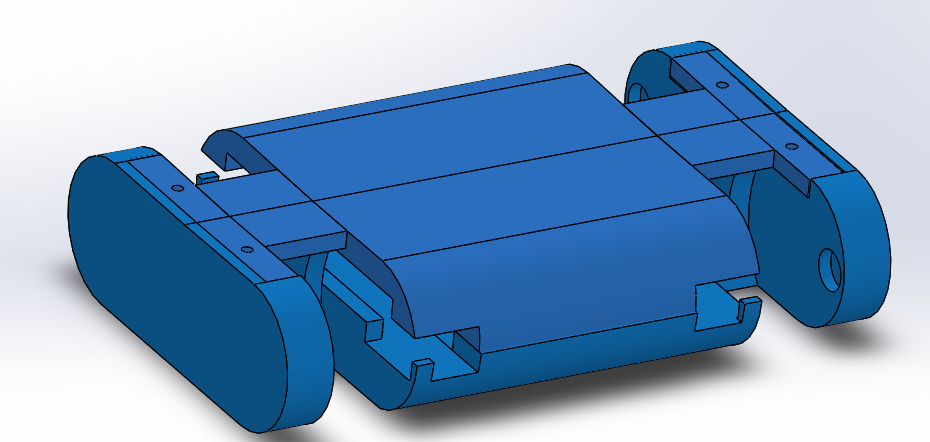
\includegraphics[width=0.6\textwidth]{img/fig12-c-body.png}
    \caption{Thiết kế thân liền khối nhằm đạt độ bền cao và khối lượng nhẹ.}
    \label{fig12-c}
\end{figure}

\begin{figure}[H]
    \centering
    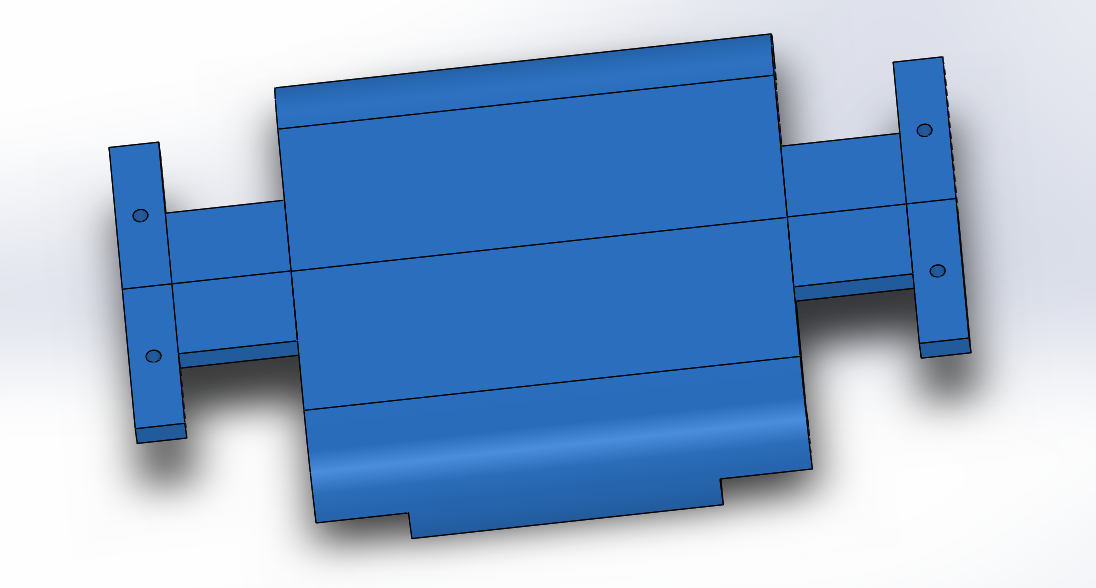
\includegraphics[width=0.6\textwidth]{img/fig12-b-nắp thân.png}
    \caption{Nắp thân.}
    \label{fig12-b}
\end{figure}

\begin{figure}[H]
    \centering
    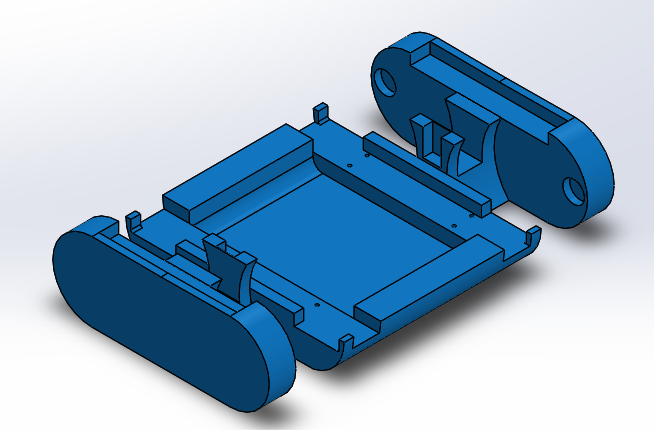
\includegraphics[width=0.6\textwidth]{img/fig12-a-thân.png}
    \caption{Thiết kế thân.}
    \label{fig12-a}
\end{figure}


\subsection{Thiết kế khớp hông}

Khớp hông của robot bốn chân được thiết kế để tạo ra hai bậc tự do, một cho chuyển động roll và một cho chuyển động pitch. Mỗi chuyển động được truyền động bởi một servo.

Do servo được sử dụng trong thiết kế của chúng tôi là loại servo một trục, các ổ bi mặt bích 626zz được sử dụng ở phía đối diện trục servo nhằm giảm lực hướng kính tác dụng lên trục. Đầu trục và khớp hông được tích hợp trong quá trình chế tạo, điều này giúp thuận tiện cho việc lắp đặt và giảm sai số lắp ráp.

Ngoài ra, servo điều khiển chuyển động vung trước (tức là chuyển động pitch) của khớp hông được lắp bên trong giá đỡ khớp hông để tiết kiệm không gian. Mô hình 3D của cụm khớp hông được thể hiện trong Hình \ref{fig13}.

\begin{figure}[H]
    \centering
    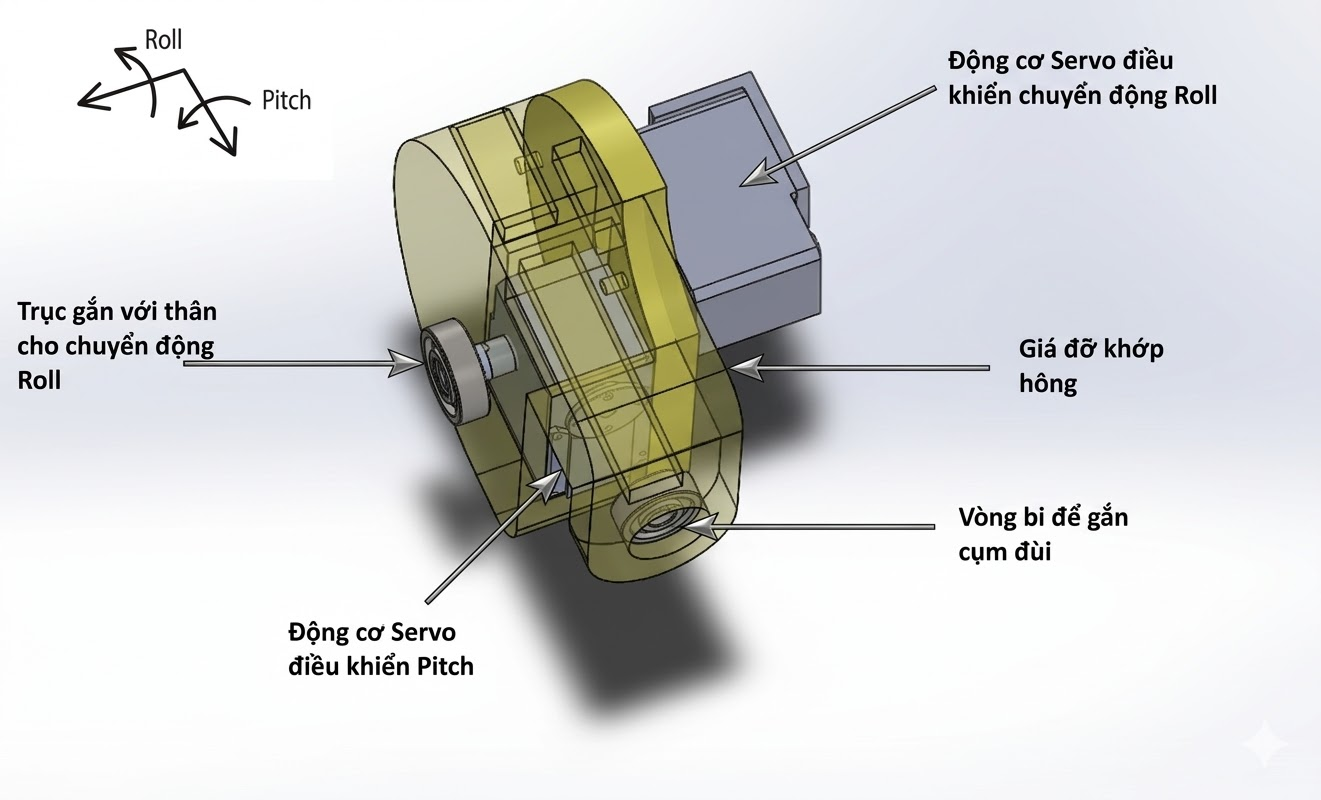
\includegraphics[width=0.6\textwidth]{img/fig13-Hip-joint assembly for the lateral and longitudinal swing motions..jpg }
    \caption{Cụm khớp hông cho chuyển động vung ngang và vung dọc.}
    \label{fig13}
\end{figure}

\subsection{Thiết kế chân}

Chân của robot bốn chân thường xuyên tiếp xúc với mặt đất để tạo lực đẩy, do đó thiết kế chân đóng vai trò quan trọng đối với khả năng di chuyển thành công của robot.

Chuyển động vung trước của khớp hông (phần đùi) sử dụng ổ bi để chịu lực dọc trục. Vì khối lượng của chân đã được bỏ qua trong các tính toán động học trình bày bên dưới, nên phần đùi và cẳng chân cần được thiết kế sao cho khối lượng và mô men quán tính nhỏ nhất có thể nhằm giảm sai số lý thuyết.

Trong thiết kế này, thay vì sử dụng kết nối servo trực tiếp tại khớp gối, một cơ cấu liên kết đầu bi (ball-head linkage) được sử dụng, trong đó cẳng chân được truyền động gián tiếp thông qua tay đòn (rocker arm) của servo. Cách bố trí này cho phép đặt servo ở phía trên của đùi, gần khớp hông, nơi mô men quán tính quay của chân tương đối nhỏ.

Mô hình lắp ráp một chân đơn được thể hiện trong Hình \ref{fig14}.

\begin{figure}[H]
    \centering
    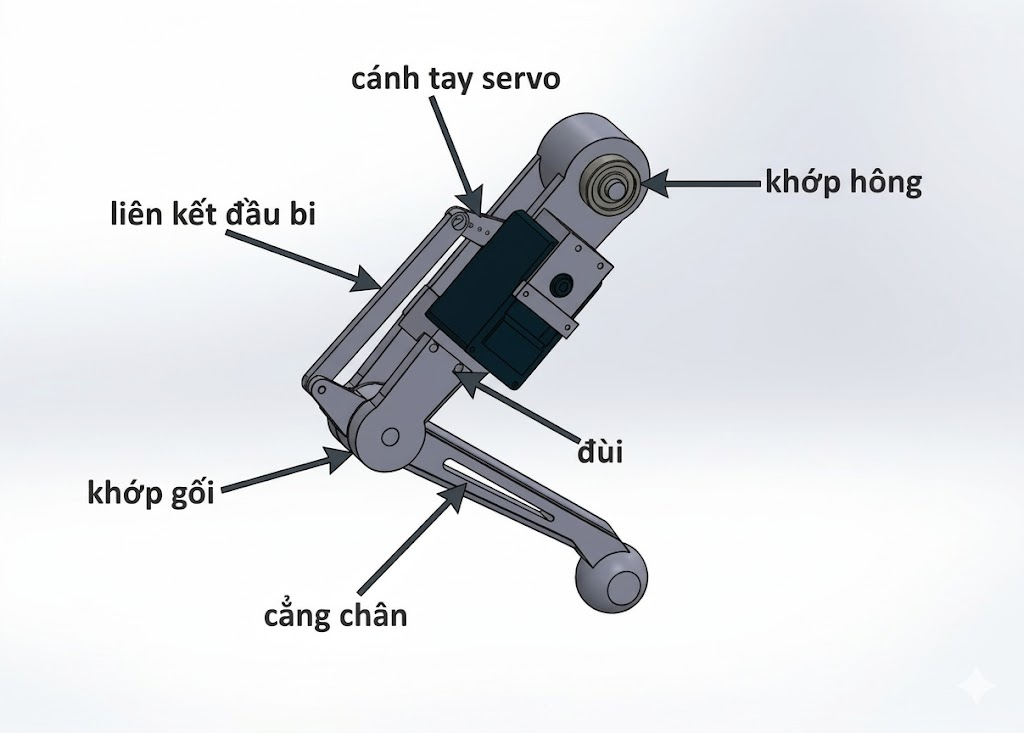
\includegraphics[width=0.6\textwidth]{img/fig14- Single leg assembly..jpg}
    \caption{Cụm lắp ráp một chân đơn.}
    \label{fig14}
\end{figure}

Dựa trên cấu trúc chân của robot bốn chân, có thể thấy rằng cẳng chân là bộ phận dễ bị gãy và uốn cong nhất vì nó phải chịu trọng lượng của toàn bộ robot cũng như các lực nén khi tiếp xúc với mặt đất. 

Ở đây, lực tiếp xúc với mặt đất được đơn giản hóa chỉ gồm lực pháp tuyến $F_N$ và lực tiếp tuyến $F_\mu$ trong mặt phẳng thẳng đứng, như thể hiện ở Hình \ref{fig15}.

Khi cẳng chân quay quanh trục khớp gối, nếu bỏ qua ma sát tại khớp và ma sát tiếp xúc với mặt đất, mô-men tải ngoài lớn nhất có thể được xác định theo công thức:

\begin{equation}
    T_{\text{max}} = \eta F_N L_3 \sin(\alpha)
\end{equation}

trong đó $F_N$ là lực pháp tuyến, $L_3$ là khoảng cách từ trục khớp gối đến điểm tiếp xúc mặt đất, $\alpha$ là góc giữa cẳng chân và phương thẳng đứng và $\eta$ là hệ số tải động.

Bằng cách định nghĩa các thuộc tính vật liệu phù hợp cho từng bộ phận của robot bốn chân trong mô hình SolidWorks, tổng khối lượng robot thu được xấp xỉ $M = 2.3\text{ kg}$.

Giả sử bốn chân chịu đều toàn bộ trọng lượng của robot trong trạng thái tĩnh, lực pháp tuyến được tính là:

\begin{equation}
    F_N = \frac{Mg}{4}
\end{equation}

Trong phân tích bền số học dưới đây, sử dụng các giá trị: chiều dài cẳng chân $L_3 = 0.125\text{ m}$, góc nghiêng $\alpha = 45^\circ$, và hệ số tải động $\eta = 1.2$.

\section{Phân tích vật liệu và công nghệ chế tạo}

\subsection{Lựa chọn vật liệu in 3D}

Toàn bộ các chi tiết cơ khí của robot (thân, giá đỡ khớp hông, đùi, cẳng chân) được chế tạo bằng công nghệ in 3D FDM (Fused Deposition Modeling). Vật liệu được lựa chọn là PLA (Polylactic Acid) --- một loại nhựa sinh học phổ biến trong prototyping nhanh. Bảng~\ref{tab:pla_props} trình bày các thuộc tính cơ học chính của PLA so với một số vật liệu thay thế.

\begin{table}[H]
\centering
\caption{So sánh thuộc tính cơ học các vật liệu in 3D phổ biến}
\label{tab:pla_props}
\renewcommand{\arraystretch}{1.3}
\begin{tabular}{|l|c|c|c|c|}
\hline
\textbf{Thuộc tính} & \textbf{PLA} & \textbf{ABS} & \textbf{PETG} & \textbf{Nylon} \\ \hline
Giới hạn bền kéo (MPa) & 50--60 & 35--45 & 50--55 & 70--85 \\ \hline
Mô đun đàn hồi (GPa) & 3,5 & 2,1 & 2,0 & 1,5--2,5 \\ \hline
Tỷ trọng (g/cm$^3$) & 1,24 & 1,04 & 1,27 & 1,14 \\ \hline
Nhiệt độ biến dạng ($^\circ$C) & 56 & 98 & 72 & 180 \\ \hline
Độ khó in & Thấp & Trung bình & Trung bình & Cao \\ \hline
Giá thành & Thấp & Trung bình & Trung bình & Cao \\ \hline
\end{tabular}
\end{table}

PLA được chọn vì các lý do sau:
\begin{itemize}
    \item \textbf{Độ cứng cao:} Mô đun đàn hồi $E = 3{,}5$ GPa là cao nhất trong các vật liệu in 3D phổ biến, giúp giảm biến dạng dưới tải trọng.
    \item \textbf{Dễ in:} Nhiệt độ đùn thấp ($200$--$210^\circ$C), không cần bàn sấy nóng, ít cong vênh (warping).
    \item \textbf{Chi phí thấp:} Phù hợp với giai đoạn prototyping và nghiên cứu.
    \item \textbf{Bề mặt mịn:} Chất lượng bề mặt tốt, giảm ma sát tại các vùng tiếp xúc khớp.
\end{itemize}

Tuy nhiên, PLA có nhược điểm là giòn (dễ gãy khi va đập mạnh) và chịu nhiệt kém (biến dạng trên $56^\circ$C). Để khắc phục, các vùng chịu lực tập trung (như đầu nối khớp hông) được in với mật độ điền (infill density) 80--100\%, cao hơn so với mức 30--40\% thông thường.

\subsection{Tham số in 3D}

Bảng~\ref{tab:print_params} trình bày các tham số in 3D được sử dụng để chế tạo các chi tiết cơ khí.

\begin{table}[H]
\centering
\caption{Tham số in 3D cho các chi tiết robot}
\label{tab:print_params}
\renewcommand{\arraystretch}{1.3}
\begin{tabular}{|l|c|l|}
\hline
\textbf{Tham số} & \textbf{Giá trị} & \textbf{Ghi chú} \\ \hline
Chiều cao lớp in (layer height) & 0,2 mm & Cân bằng tốc độ và chất lượng \\ \hline
Số vỏ ngoài (wall count) & 4 & Tăng độ bền \\ \hline
Mật độ điền -- thân & 40\% & Pattern: gyroid \\ \hline
Mật độ điền -- khớp & 80--100\% & Chịu lực tập trung \\ \hline
Nhiệt độ đùn & 210$^\circ$C & PLA+ \\ \hline
Tốc độ in & 50 mm/s & Đảm bảo bám dính lớp \\ \hline
Hỗ trợ (support) & Có & Cho các góc nhô > 45$^\circ$ \\ \hline
\end{tabular}
\end{table}

Tổng thời gian in cho toàn bộ chi tiết robot (thân, nắp thân, 4 bộ khớp hông, 4 đùi, 4 cẳng chân, phụ kiện) là khoảng 35--40 giờ. Sau khi in, các chi tiết được xử lý hậu kỳ: loại bỏ support, chà nhám bề mặt tiếp xúc khớp, và khoan lỗ cho ốc vít M3 cùng ổ bi 626zz.

\subsection{Phân tích tải trọng bằng SolidWorks Simulation}

Để kiểm chứng độ bền của thiết kế, nhóm đã thực hiện phân tích phần tử hữu hạn (FEA -- Finite Element Analysis) trên phần mềm SolidWorks Simulation cho chi tiết cẳng chân --- bộ phận chịu tải lớn nhất. Các điều kiện biên được đặt là:

\begin{itemize}
    \item \textbf{Ràng buộc:} Cố định đầu trên cẳng chân (vùng nối với khớp gối).
    \item \textbf{Tải trọng:} Lực pháp tuyến $F_N = 11{,}28$ N tại đầu dưới cẳng chân (bàn chân), hướng dọc theo trục chân.
    \item \textbf{Vật liệu:} PLA với $E = 3{,}5$ GPa, $\sigma_{yield} = 50$ MPa.
\end{itemize}

Kết quả phân tích cho thấy ứng suất Von Mises cực đại trên cẳng chân đạt khoảng $12$ MPa, nhỏ hơn nhiều so với giới hạn chảy $50$ MPa của PLA, cho hệ số an toàn $n = 50/12 \approx 4{,}2$. Giá trị này xác nhận thiết kế cẳng chân đủ bền cho vận hành bình thường.

\section{Lựa chọn cơ cấu chấp hành}
Việc lựa chọn cơ cấu chấp hành có ảnh hưởng lớn đến hiệu năng di chuyển của robot bốn chân. Do trọng lượng bản thân của robot, cơ cấu chấp hành cần tạo ra mô-men xoắn lớn, đáp ứng nhanh và có kích thước nhỏ gọn.

Động cơ không chổi than được sử dụng rộng rãi nhờ đặc tính động học vượt trội, tuy nhiên chúng thường có giá thành cao và kích thước lớn.

Vì trọng tâm chính của đồ án này là triển khai và đánh giá sơ bộ thuật toán dáng đi trên mô hình robot kích thước để bàn, nên servo được lựa chọn làm nguồn truyền động.

Được trang bị khả năng phản hồi góc quay trực tiếp theo thời gian thực cùng tỷ số truyền bánh răng lớn, loại servo này cho phép vi điều khiển dễ dàng thực hiện điều khiển vòng kín. Điều này là nền tảng thiết yếu để chạy các node tính toán động học nghịch, giúp robot tự bù trừ sai số trong các thử nghiệm dáng đi phức tạp và tự cân bằng chính xác hơn.

Mẫu servo được sử dụng là ST3215 và ST3215-HS, như thể hiện ở Hình \ref{fig16}, và các thông số kỹ thuật cụ thể được trình bày trong Bảng \ref{tab:1}.

\begin{figure}[H]
    \centering
    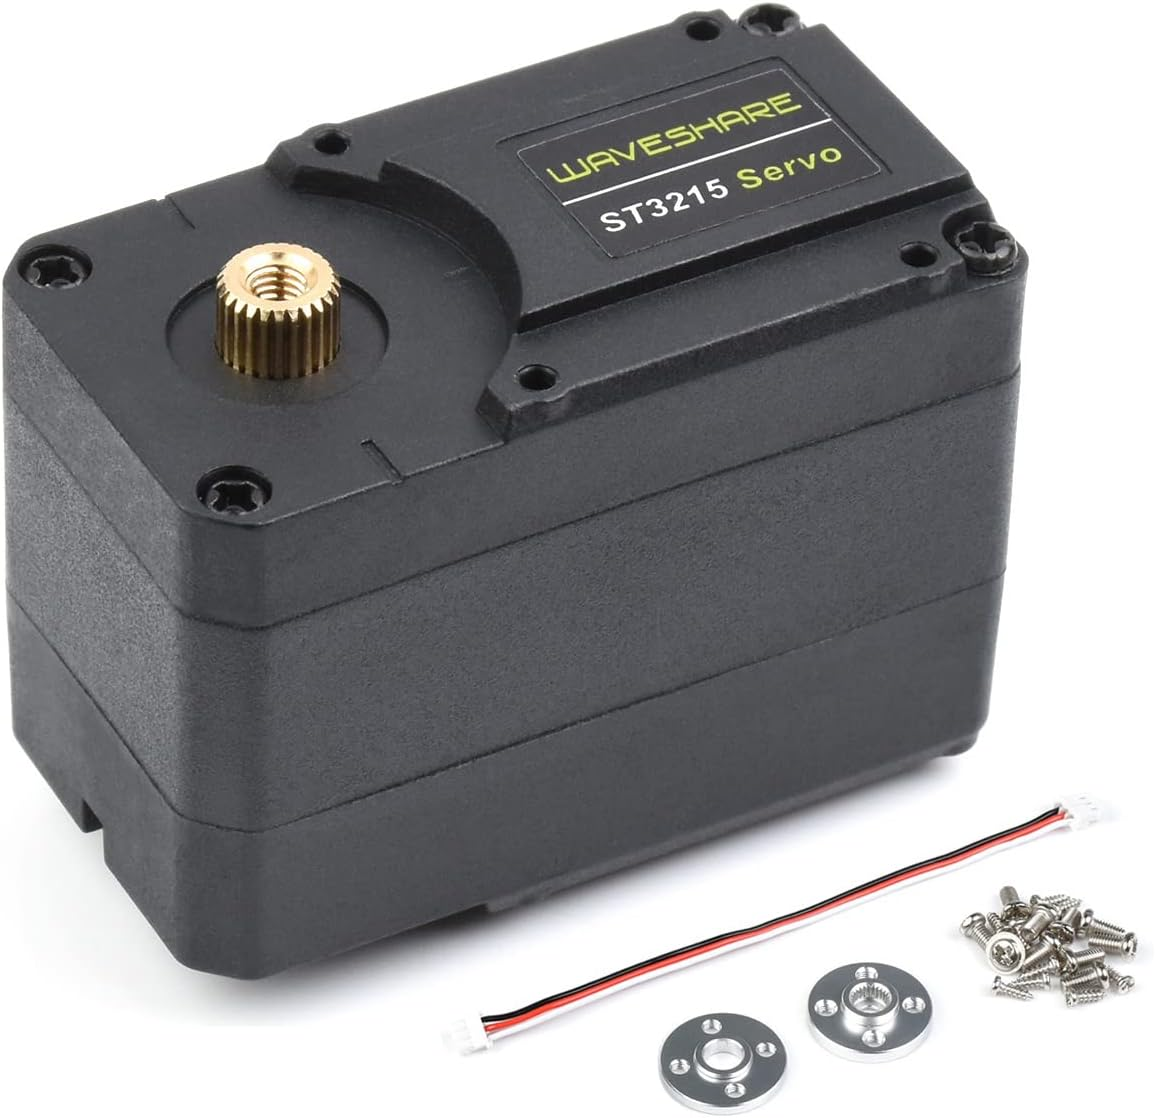
\includegraphics[width=0.6\textwidth]{img/fig16-ST3215.jpg}
    \caption{Cơ cấu chấp hành servo ST3215 dùng cho robot bốn chân.}
    \label{fig16}
\end{figure}

\begin{table}[htbp]
    \centering
    \caption{Thông số kỹ thuật của động cơ servo ST3215 và ST3215-HS.}
    \label{tab:1}
    \resizebox{\textwidth}{!}{% Thu nhỏ bảng vừa với chiều rộng trang giấy
        \begin{tabular}{l c c c c c c c}
            \toprule
            \textbf{Mẫu} & \textbf{Trọng lượng} & \textbf{\makecell{Kích thước \\ (L $\times$ W $\times$ H)}} & \textbf{\makecell{Điện áp \\ hoạt động}} & \textbf{\makecell{Tốc độ truyền \\ (Baudrate)}} & \textbf{\makecell{Phạm vi \\ góc quay}} & \textbf{Tốc độ tối đa} & \textbf{Lực xoắn tối đa} \\
            \midrule
            ST3215 & 69 g & \makecell{$45.2 \times 24.7 \times$ \\ $35.0$ mm} & 6.0 V -- 12.6 V & \textasciitilde 1 Mbps & \makecell{360$^\circ$ } & 0.222 s/60$^\circ$ (@12 V) & 30 kg$\cdot$cm (@12 V) \\
            \addlinespace % Thêm một khoảng trắng nhỏ giữa 2 hàng cho thoáng
            ST3215-HS & 68 g & \makecell{$45.2 \times 24.7 \times$ \\ $35.0$ mm} & 6.0 V -- 12.6 V & \textasciitilde 1 Mbps & \makecell{360$^\circ$ } & 0.094 s/60$^\circ$ (@12 V) & 20 kg$\cdot$cm (@12 V) \\
            \bottomrule
        \end{tabular}
    }
\end{table}

Để kiểm chứng mô-men xoắn định mức của servo đã chọn, tiến hành phân tích như sau. Dựa trên phân tích ở Mục 3.1.3, ảnh hưởng của mô-men xoắn lên cẳng chân là đáng kể nhất. Gọi góc giữa lực pháp tuyến tiếp xúc mặt đất $F_N$ và cẳng chân $L_3$ là $\alpha$. Như thể hiện trong Hình \ref{fig17}, mô-men do lực tiếp đất tác dụng lên khớp gối là:
\begin{equation}
    M_{\text{knee}} = \eta F_N L_3 \sin(\alpha)
\end{equation}
Mô-men này được cân bằng bởi lực truyền $F_t$ dọc theo thanh liên kết $CD$:
\begin{equation}
    M_{\text{knee}} = F_t L_{CB} \sin(\gamma)
\end{equation}
với $\gamma$ là góc giữa thanh liên kết $CD$ và cánh tay đòn $CB$. Mô-men tác dụng lên trục servo (qua cánh tay đòn $DE$) là:
\begin{equation}
    T_{\text{knee}} = F_t L_{DE} \sin(\beta)
\end{equation}
với $\beta$ là góc giữa thanh $CD$ và tay đòn $DE$. Trong thiết kế cơ cấu gần với hình bình hành, $\gamma \approx \beta$, do đó tỉ số $\sin(\beta)/\sin(\gamma) \approx 1$. Từ đó ta suy ra mô-men yêu cầu tại servo cẳng chân là:
\begin{equation}
    T_{\text{knee}} \approx \eta F_N L_3 \sin(\alpha) \frac{L_{DE}}{L_{CB}}
\end{equation}
Trong dáng đi trot, luôn có hai chân tiếp xúc mặt đất, do đó tải trọng lớn nhất tác dụng lên một chân là:
\begin{equation}
    F_N = \frac{Mg}{2}
\end{equation}
Thay các giá trị từ Bảng \ref{tab:2} với $M = 2.3\,\text{kg}$, $L_3 = 0.125\,\text{m}$, $L_{DE} = 0.024\,\text{m}$, $L_{CB} = 0.025\,\text{m}$, hệ số tải động $\eta = 1.2$, góc nghiêng $\alpha = 45^\circ$, và $g = 9.81\,\text{m/s}^2$ vào công thức, ta có $F_N = 11.28\,\text{N}$ và:
\begin{equation}
    T_{\text{knee}} \approx 1.2 \times 11.28 \times 0.125 \times \sin(45^\circ) \times \frac{0.024}{0.025} \approx 1.149\,\text{N}\cdot\text{m} \approx 11.7\,\text{kg}\cdot\text{cm}
\end{equation}

Giá trị này nhỏ hơn mô-men định mức $20\,\text{kg}\cdot\text{cm}$ của servo ST3215-HS, đảm bảo động cơ hoạt động an toàn.

\begin{figure}[H]
    \centering
    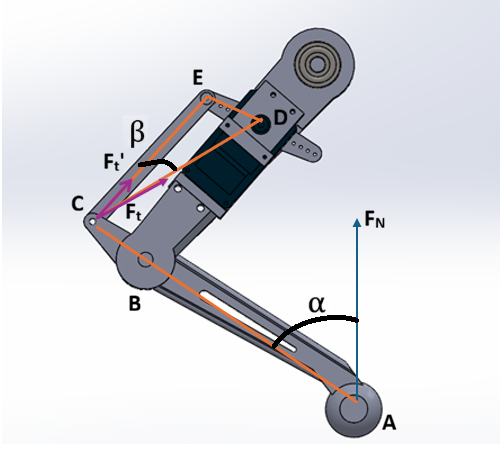
\includegraphics[width=0.6\textwidth]{img/fig17-Torque analysis of the lower leg servo actuator.png}
    \caption{Phân tích mô-men xoắn của cơ cấu chấp hành servo tại cẳng chân.}
    \label{fig17}
\end{figure}

\subsection{Phân tích mô-men khớp vai (Hip Roll)}

Trong thực tế vận hành, để duy trì khả năng thăng bằng và giảm chấn, chân robot không bao giờ duỗi thẳng hoàn toàn. Thay vào đó, phần đùi ($L_2$) và cẳng chân ($L_3$) luôn tạo với nhau một góc gập nhất định như thể hiện ở Hình \ref{fig18}. Việc tính toán mô-men xoắn cần sử dụng khoảng cách thực tế từ khớp hông đến bàn chân. 

Gọi $L_{hd}$ là khoảng cách hiệu dụng từ trục khớp hông đến điểm tiếp xúc mặt đất của bàn chân. Dựa trên định lý hàm số cosin cho tam giác tạo bởi đùi, cẳng chân và góc gập gối $\beta$, ta có:
\begin{equation}
    L_{hd} = \sqrt{L_2^2 + L_3^2 - 2L_2L_3\cos(\beta)}
\end{equation}

Dựa theo Bảng \ref{tab:2} với thiết kế $L_2 = 0.106\,\text{m}$ và $L_3 = 0.125\,\text{m}$, giả sử ở tư thế đi bộ trot tiêu chuẩn robot duy trì góc khuỵu gối $\beta = 90^\circ$ nhằm tối ưu lực bám. Chiều dài hiệu dụng lúc này là:
\begin{equation}
    L_{hd} = \sqrt{0.106^2 + 0.125^2 - 2(0.106)(0.125)\cos(90^\circ)} \approx 0.164\,\text{m}
\end{equation}

Tương tự phân tích trước, tải trọng lớn nhất tác dụng lên một chân là $F_N = 11.28\,\text{N}$, hệ số tải động $\eta = 1.2$, dẫn đến lực tác dụng tổng cộng là $\eta F_N = 13.54\,\text{N}$. 

Công thức tính mô-men xoắn cực đại cho khớp vai $T_{roll}$ theo góc dang chân $\theta_1$ được xác định dựa trên khoảng lệch ngàm $L_1$ và hình chiếu ngang của chiều dài chân hiệu dụng:
\begin{equation}
    T_{roll} = \eta F_N \big(L_1 \cos(\theta_1) + L_{hd} \sin(\theta_1)\big)
\end{equation}

Thay các thông số thiết kế ($L_1 = 0.026\,\text{m}$) vào phương trình, ta thu được:
\begin{equation}
    T_{roll} = 13.54 \times \big(0.026 \cos(\theta_1) + 0.164 \sin(\theta_1)\big) \quad \text{(N}\cdot\text{m)}
\end{equation}

\begin{itemize}
    \item Khi $\theta_1 = 0^\circ$, mô-men tác dụng lên khớp vai chỉ xuất phát từ khoảng lệch ngàm cơ khí: $T_{roll} = 13.54 \times 0.026 \approx 0.35\,\text{N}\cdot\text{m} \approx 3.6\,\text{kg}\cdot\text{cm}$.
    \item Khi $\theta_1 = 15^\circ$, mô-men tăng lên: $T_{roll} \approx 0.91\,\text{N}\cdot\text{m} \approx 9.3\,\text{kg}\cdot\text{cm}$, phản ánh trạng thái robot điều chỉnh tư thế rẽ với góc dang trung bình.
    \item Khi $\theta_1 = 30^\circ$, mô-men đạt giá trị lớn nhất: $T_{roll} \approx 1.41\,\text{N}\cdot\text{m} \approx 14.4\,\text{kg}\cdot\text{cm}$, tương ứng với tình huống bất lợi khi chân dang rộng.
\end{itemize}

Giá trị mô-men cực đại vẫn nhỏ hơn định mức $20\,\text{kg}\cdot\text{cm}$ của servo ST3215-HS, do đó khớp vai vẫn hoạt động trong vùng an toàn, không gây quá tải.

\begin{figure}[H]
    \centering
    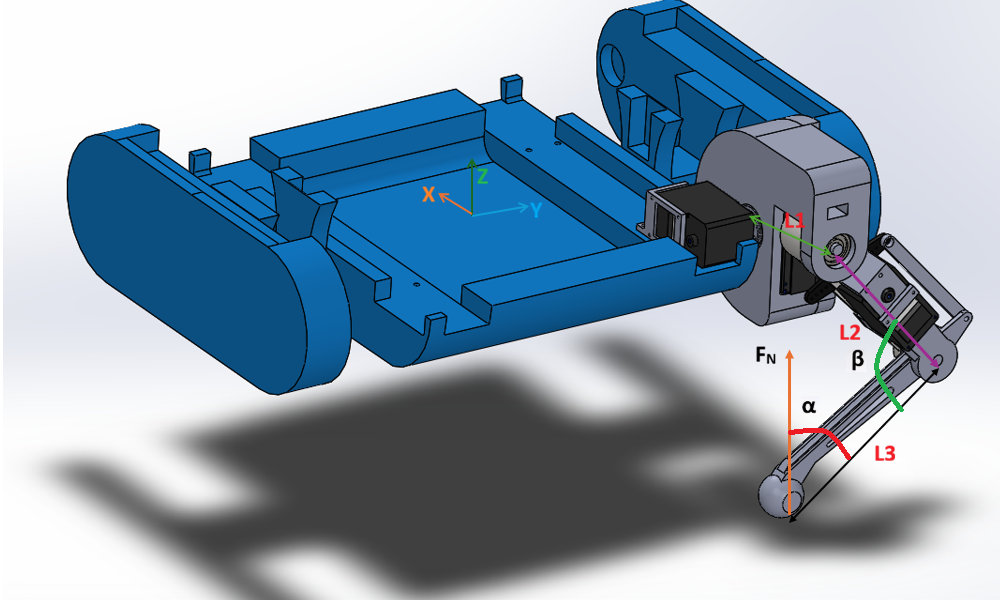
\includegraphics[width=0.6\textwidth]{img/fig18-Free body diagram.png}
    \caption{Mô hình một chân của robot bốn chân.}
    \label{fig18}
\end{figure}

\subsection{Phân tích mô-men khớp hông (Hip Pitch)}

Tương tự quy trình đánh giá ở khớp vai, mô-men xoắn yêu cầu cực đại đối với khớp hông (Pitch) được xác định thông qua chiều dài sải bước hiệu dụng của robot. Trong mặt phẳng dọc, cánh tay đòn tạo ra mô-men phụ thuộc vào độ vươn xa của bàn chân theo phương ngang. Gọi $\alpha$ là góc nghiêng của chân (đường nối từ trục khớp hông đến bàn chân) so với phương thẳng đứng. Phương trình tổng quát tính mô-men xoắn cho khớp hông là:
\begin{equation}
    T_{pitch} = \eta F_N L_{hd} \sin(\alpha)
\end{equation}

Sử dụng khoảng cách hiệu dụng $L_{hd} = 0.164\,\text{m}$ và lực tải $\eta F_N = 13.54\,\text{N}$ đã xác định:
\begin{equation}
    T_{pitch} = 13.54 \times 0.164 \sin(\alpha) = 2.221 \sin(\alpha) \quad \text{(N}\cdot\text{m)}
\end{equation}

Phân tích quỹ đạo chuyển động cho thấy:
\begin{itemize}
    \item Tại tư thế đứng thẳng chân ($\alpha = 0^\circ$), trọng lượng truyền dọc theo chân nên khớp hông không chịu tải uốn ($T_{pitch} = 0$).
    \item Khi chân bước với góc $\alpha = 15^\circ$, mô-men tại khớp hông đạt $T_{pitch} = 2.221 \sin(15^\circ) \approx 0.57\,\text{N}\cdot\text{m} \approx 5.9\,\text{kg}\cdot\text{cm}$. Đây là vùng tải nhẹ, thuận lợi cho động cơ.
    \item Khi $\alpha = 45^\circ$, mô-men tăng lên $T_{pitch} = 2.221 \sin(45^\circ) \approx 1.57\,\text{N}\cdot\text{m} \approx 16.0\,\text{kg}\cdot\text{cm}$, tương ứng với trạng thái vươn dài chân để leo dốc hoặc vượt chướng ngại vật.
\end{itemize}

Giá trị cực đại này vẫn nhỏ hơn đáng kể so với giới hạn mô-men của servo ST3215-HS, xác nhận rằng việc lựa chọn động cơ cho khớp hông là hoàn toàn phù hợp và đảm bảo độ tin cậy trong vận hành.

\subsection{Thiết kế tổng thể}

Thiết kế tổng thể của robot bốn chân được thể hiện trong Hình \ref{fig19}, với tổng cộng 12 bậc tự do và cấu hình chân full-elbow. Ở đây, cả bốn chân đều giống hệt nhau về cấu trúc và kích thước nhằm tạo thuận lợi cho việc điều khiển.

Khớp hông được kết nối trực tiếp với servo ở cả hai bậc tự do để đơn giản hóa cấu trúc bên trong, trong khi khớp gối được thiết kế sử dụng cơ cấu tay đòn servo kết hợp với thanh liên kết nhằm giảm quán tính của chân.

Các tham số chính của hệ thống được trình bày trong Bảng \ref{tab:2}.

\begin{figure}[H]
    \centering
    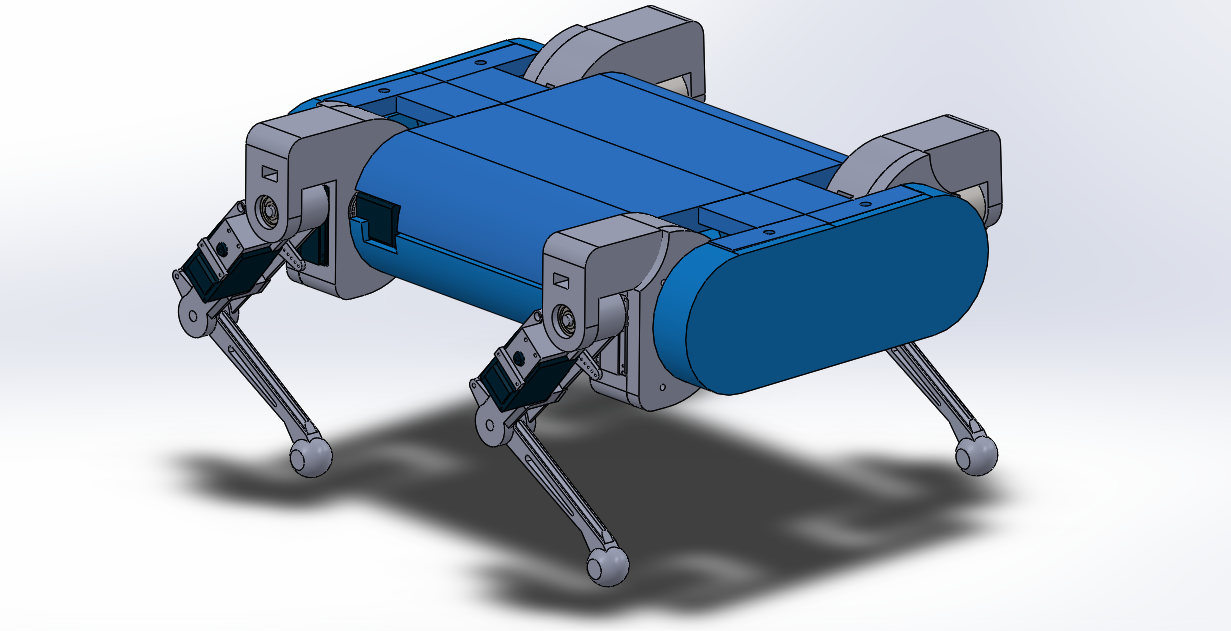
\includegraphics[width=0.6\textwidth]{img/fig19-preview_design.png }
    \caption{3D thiết kế robot Dog}
    \label{fig19}
\end{figure}

\begin{table}[h]
\centering
\caption{Các thông số chính của robot bốn chân}
 \label{tab:2}
\begin{tabular}{ccccccc}
\toprule
Chiều dài & Chiều rộng & Chiều cao & \makecell{Chiều dài\\hông\\$L_1$} & \makecell{Chiều dài\\đùi\\$L_2$} & \makecell{Chiều dài\\cẳng chân\\$L_3$} & \makecell{Bậc\\tự do} \\
\midrule
209 mm & 191 mm & 185 mm & 26 mm & 106 mm & 125 mm & 12 \\
\bottomrule
\end{tabular}
\end{table}

\subsection{Phân tích ngân sách khối lượng}

Việc quản lý khối lượng có ý nghĩa quan trọng đối với robot bốn chân, ảnh hưởng trực tiếp đến mô-men yêu cầu tại các khớp, thời gian hoạt động và tính ổn định. Bảng~\ref{tab:weight_budget} trình bày phân tích chi tiết ngân sách khối lượng của toàn bộ hệ thống.

\begin{table}[H]
\centering
\caption{Ngân sách khối lượng robot bốn chân}
\label{tab:weight_budget}
\renewcommand{\arraystretch}{1.3}
\begin{tabular}{|l|c|c|c|}
\hline
\textbf{Thành phần} & \textbf{Số lượng} & \textbf{Đơn vị (g)} & \textbf{Tổng (g)} \\ \hline
Khung thân (PLA) & 1 & 250 & 250 \\ \hline
Nắp thân (PLA) & 1 & 80 & 80 \\ \hline
Cụm khớp hông (PLA) & 4 & 45 & 180 \\ \hline
Đùi chân (PLA) & 4 & 30 & 120 \\ \hline
Cẳng chân (PLA) & 4 & 25 & 100 \\ \hline
Servo ST3215 & 12 & 69 & 828 \\ \hline
Jetson Nano B01 & 1 & 140 & 140 \\ \hline
IMU BNO055 & 1 & 5 & 5 \\ \hline
Bus Servo Adapter (A) & 2 & 15 & 30 \\ \hline
Mạch giảm áp XL4015 & 1 & 25 & 25 \\ \hline
Ốc vít, ổ bi, phụ kiện & -- & -- & 100 \\ \hline
Cáp và dây nối & -- & -- & 150 \\ \hline
\midrule
\textbf{Tổng cộng} & & & \textbf{$\sim$2008} \\ \hline
\end{tabular}
\end{table}

Kết quả cho thấy khối lượng robot (không bao gồm nguồn và cáp nguồn) vào khoảng 2,0 kg, phù hợp với giá trị $M = 2{,}3$ kg đã sử dụng trong các tính toán mô-men ở các mục trước (bao gồm cả cáp nguồn). Phần lớn khối lượng đến từ 12 servo ($\sim$41\%), tiếp theo là khung thân và phụ kiện PLA ($\sim$36\%).

\subsection{Quy trình lắp ráp}

Quy trình lắp ráp robot bốn chân được thực hiện theo các bước tuần tự sau:

\begin{enumerate}
    \item \textbf{Lắp ráp khớp hông:} Gắn servo hip roll vào giá đỡ khớp hông, lắp ổ bi 626zz ở phía đối diện. Sau đó lắp servo hip pitch bên trong giá đỡ.
    \item \textbf{Lắp ráp chân:} Gắn servo knee (gối) vào phần trên của đùi, nối cẳng chân qua cơ cấu tay đòn và thanh liên kết ball-head.
    \item \textbf{Nối chân với thân:} Lắp 4 cụm khớp hông vào 4 góc của thân robot. Đảm bảo các trục servo hip roll song song với trục dọc thân.
    \item \textbf{Đi dây servo:} Nối cáp tín hiệu từ 12 servo về hai mạch Bus Servo Adapter. Nhóm cáp theo danh tính driver (A: chân LF+RB, B: chân LB+RF).
    \item \textbf{Lắp điện tử:} Gắn Jetson Nano, IMU BNO055, mạch giảm áp XL4015 và hai Bus Servo Adapter vào bên trong thân robot.
    \item \textbf{Kết nối nguồn:} Nối nguồn xung 12V vào hai Bus Servo Adapter (cấp cho servo) và mạch giảm áp (cấp 5V cho Jetson Nano).
    \item \textbf{Kiểm tra:} Cấp nguồn và chạy chương trình calibrate để xác minh chiều quay, ID servo và phạm vi góc quay của từng khớp.
\end{enumerate}

Toàn bộ quá trình lắp ráp từ các chi tiết in 3D đến robot hoàn chỉnh có thể vận hành mất khoảng 4--5 giờ, không bao gồm thời gian in 3D và calibrate phần mềm.
\input{chapter/chapter4-donghoc}
\chapter {Thiết kế và xây dựng hệ thống}

\section{Tổng quan về kiến trúc hệ thống }

Kiến trúc phần cứng của hệ thống robot bốn chân được xây dựng nhằm mục tiêu cung cấp nguồn năng lượng ổn định, đảm bảo khả năng xử lý thuật toán phức tạp theo thời gian thực và điều khiển đồng bộ nhiều cơ cấu chấp hành. Sơ đồ kết nối phần cứng tổng thể của mô hình thực nghiệm được thể hiện chi tiết trong Hình~\ref{fig30}.

\begin{figure}[H]
    \centering
    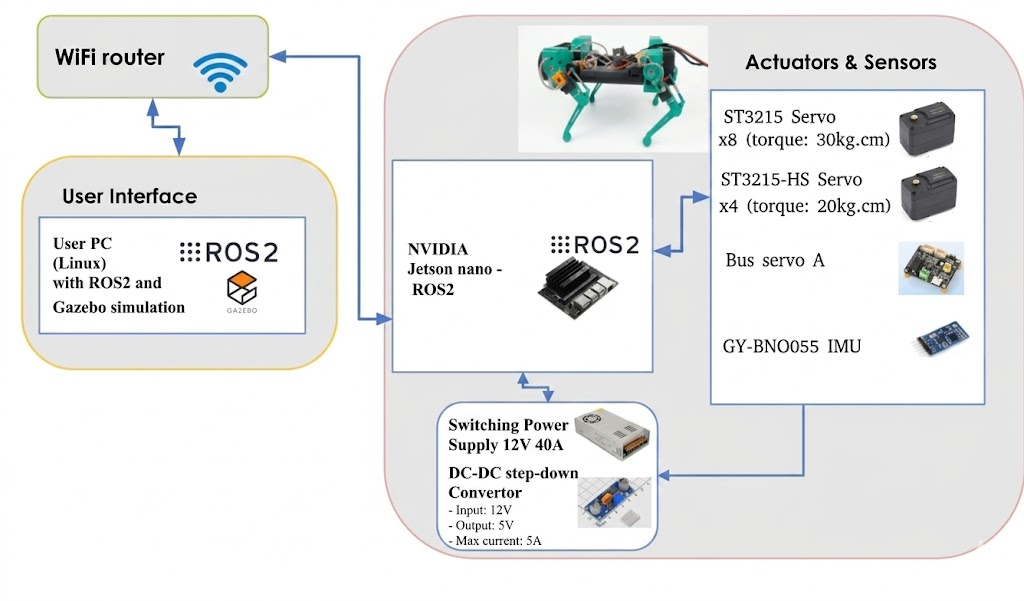
\includegraphics[width=\textwidth]{img/fig_system_overview_new.png}
    \caption{Sơ đồ kiến trúc tổng thể của hệ thống robot bốn chân.}
    \label{fig30}
\end{figure}

Hình~\ref{fig:real_robot} trình bày mô hình robot bốn chân thực tế đã được chế tạo và lắp ráp hoàn chỉnh. Robot sử dụng khung thân và các chi tiết chân được gia công bằng công nghệ in 3D FDM với vật liệu PLA, tích hợp 12 động cơ bus servo ST3215 tại các khớp, cảm biến IMU BNO055 gắn trên thân và máy tính nhúng Jetson Nano làm bộ xử lý trung tâm.

\begin{figure}[H]
    \centering
    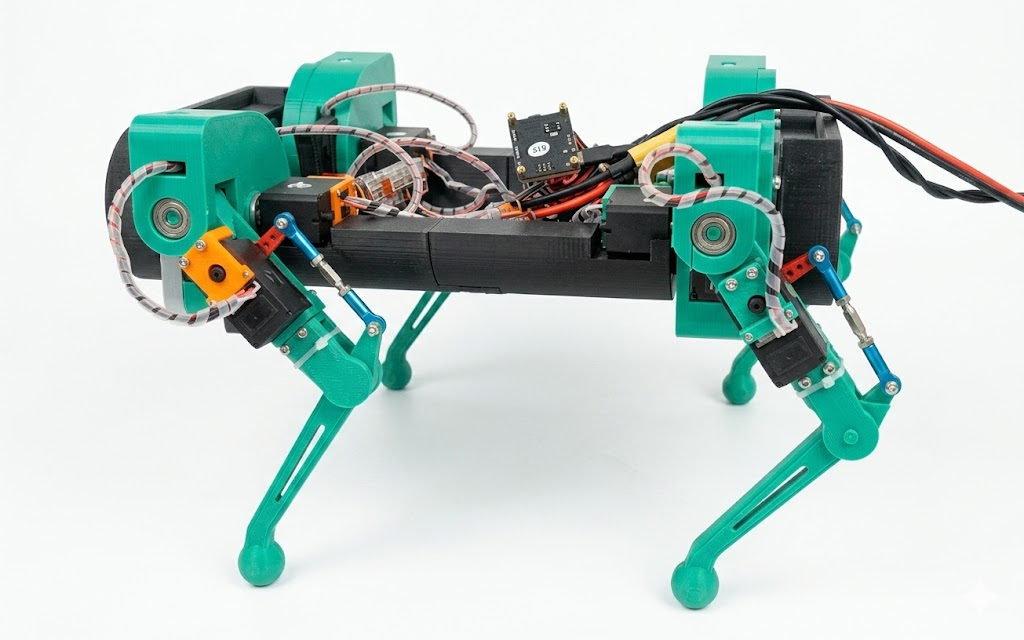
\includegraphics[width=0.85\textwidth]{img/fig_real_robot.png}
    \caption{Mô hình robot bốn chân thực tế đã được chế tạo và lắp ráp hoàn chỉnh.}
    \label{fig:real_robot}
\end{figure}

\subsection{Khối xử lý trung tâm }
Một yếu tố quan trọng của nguyên mẫu này là bộ xử lý trung tâm. Điều đầu tiên cần giải quyết là khả năng tính toán các bài toán phức tạp như động học nghịch, quy hoạch quỹ đạo và xử lý dữ liệu cân bằng theo thời gian thực.

Nhóm đã quyết định sử dụng máy tính nhúng Jetson Nano Developer Kit B01 \cite{jetson_nano} thay vì các dòng vi điều khiển phổ thông vì nó mang lại sức mạnh tính toán vượt trội hơn hẳn. Những ưu điểm này bao gồm: tốc độ xung nhịp cao từ vi xử lý Quad-core ARM Cortex-A57, tích hợp GPU mạnh mẽ, khả năng chạy hệ điều hành Linux (Ubuntu) hỗ trợ đa nhiệm, và dễ dàng tích hợp các thư viện toán học phức tạp. Nhược điểm chính của nền tảng tiên tiến này là mức tiêu thụ điện năng lớn hơn và độ phức tạp trong việc làm chủ hệ thống phần mềm.


\begin{figure}[H]
    \centering
    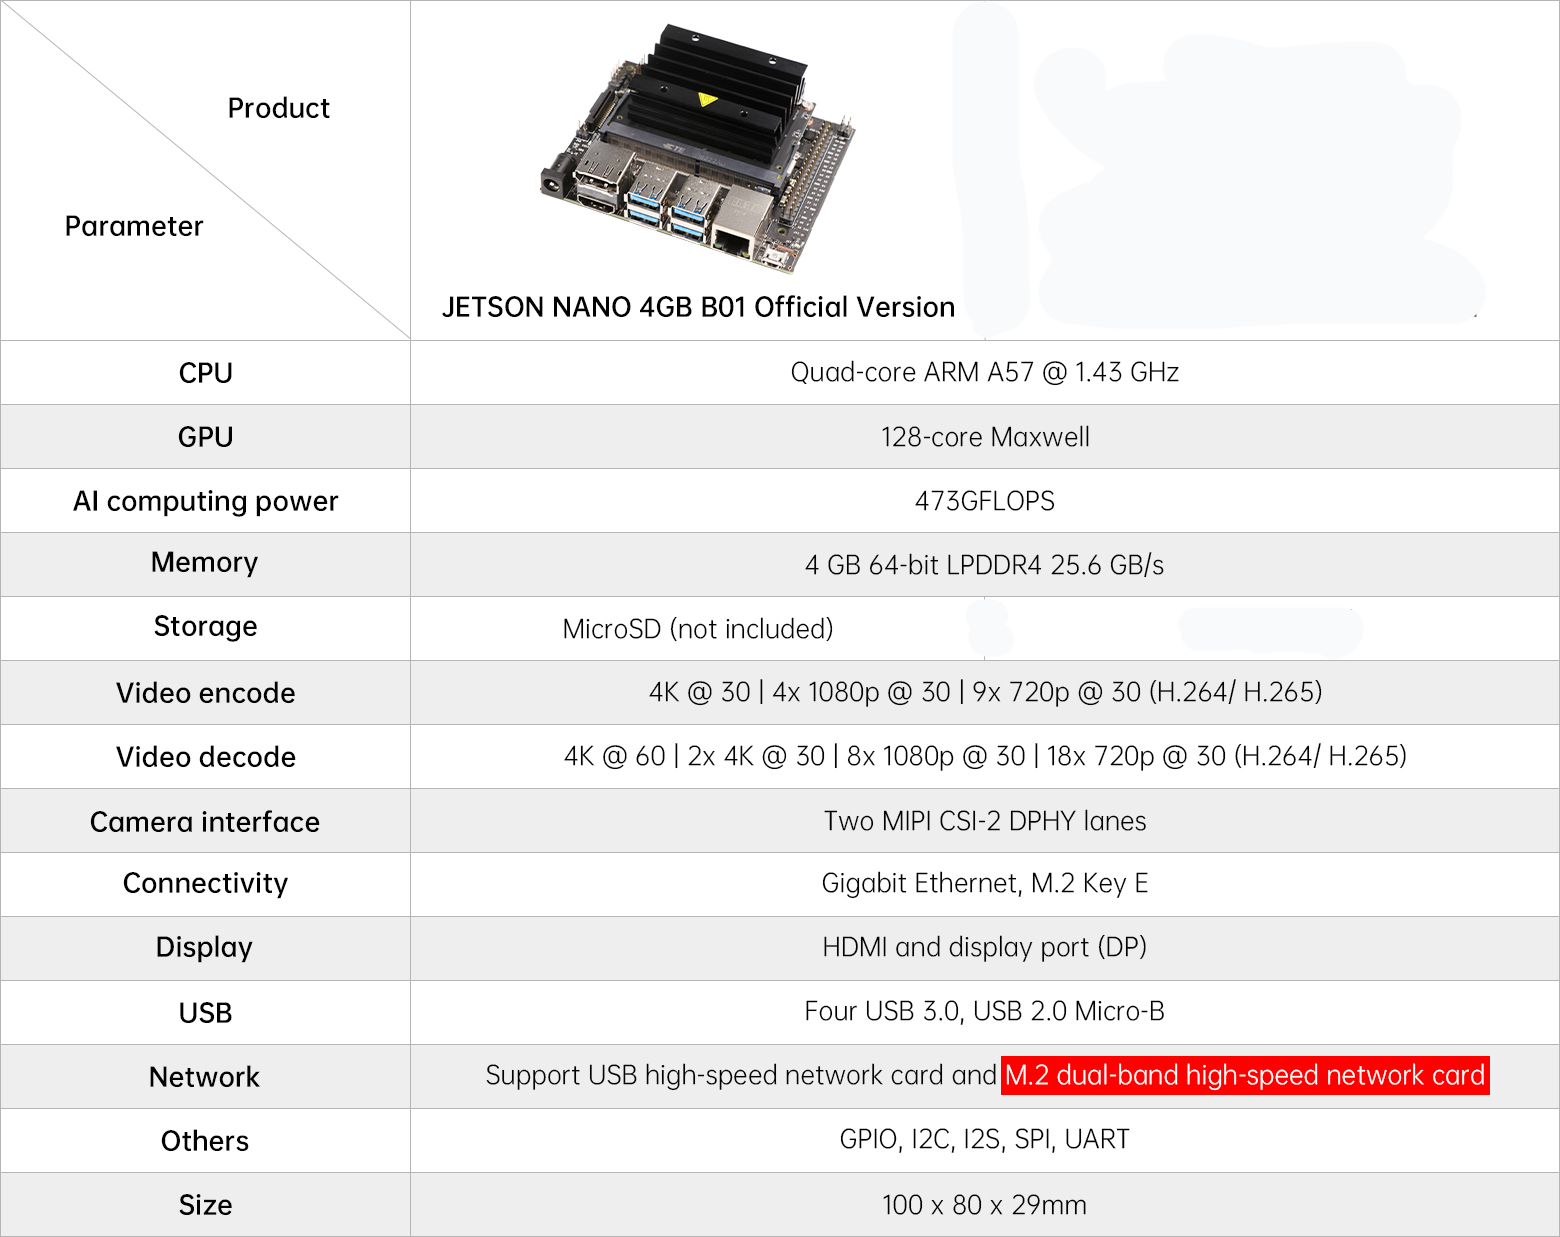
\includegraphics[width=0.8\textwidth]{img/fig34-Specifications-Jetson-B01.png} 
    \caption{Thông số kỹ thuật Jetson Nano B01}
    \label{fig34}
    \vspace{0.2cm}
\end{figure}

Hầu hết những người chế tạo robot giải trí đơn giản thường sử dụng vi điều khiển Arduino. Tuy nhiên, trong các hệ thống robot đa chân đòi hỏi khả năng giữ thăng bằng động và xử lý toán học ma trận tốc độ cao, các máy tính nhúng như dòng Jetson lại là tiêu chuẩn trong nhiều nguyên mẫu nghiên cứu. Chúng được sử dụng trong nhiều lĩnh vực, từ robot tự hành (AMR), xe tự lái đến các hệ thống AI xử lý tại biên (Edge AI) đắt tiền. Tất cả những yếu tố này đã ảnh hưởng đến quyết định của chúng em khi lựa chọn bộ xử lý cấp cao hơn cho dự án.

Jetson Nano được sử dụng để điều khiển nguyên mẫu của chúng em, bao gồm việc quản lý 12 động cơ servo và đọc dữ liệu từ module cảm biến IMU. Jetson Nano thiết lập giao tiếp UART với hai mạch Bus Servo Adapter (A). Hai mạch chuyển đổi này sẽ nhận các gói tin lệnh từ Jetson Nano và phân phối tín hiệu điều khiển nối tiếp đến 12 động cơ servo (mỗi mạch quản lý một nửa số lượng servo). Cấu trúc này giúp giảm tải dòng điện qua mạch điều khiển, phân bổ công suất hợp lý và tối giản hóa việc đi dây vật lý cho hai nửa của robot. 

\subsection{ Hệ thống Cung cấp Nguồn điện}

Sau khi nghiên cứu và lựa chọn động cơ servo ST3215 cùng mạch điều khiển, việc cấp nguồn đúng cách để hệ thống có thể đáp ứng các yêu cầu khắt khe về dòng điện tức thời trở nên vô cùng quan trọng. Để đạt được mục tiêu này, nhóm bắt đầu xem xét các phương án cung cấp năng lượng khác nhau, bao gồm pin và nguồn cấp điện trực tiếp. Các thông số kỹ thuật cốt lõi được đặt ra cho dự án bao gồm: Điện áp hoạt động, Dòng điện tối đa, Công suất tổng và Độ ổn định điện áp. Hai phương án chính được đưa ra cân nhắc là sử dụng Pin Lithium Polymer dung lượng lớn và Nguồn xung tổ ong; mỗi loại đều có những đặc tính riêng tác động đến quá trình thử nghiệm.

Trong giai đoạn phát triển, thử nghiệm thuật toán và tinh chỉnh động học, hệ thống yêu cầu một nguồn điện có khả năng cung cấp dòng xả lớn, liên tục trong nhiều giờ đồng hồ mà không xảy ra hiện tượng sụt áp. Việc khởi chạy hoặc ép tải 12 động cơ servo cùng lúc đòi hỏi dòng khởi động cực kỳ cao. Do đó, nguồn xung tổ ong 12V - 40A (480W) đã được lựa chọn làm giải pháp cung cấp năng lượng chính thay vì dùng pin. Ưu điểm lớn nhất của nguồn tổ ong là giá thành hợp lý, khả năng cấp dòng xả lên đến 40A một cách ổn định và cung cấp đúng mức điện áp 12V tối ưu cho các servo ST3215 hoạt động với hiệu suất cao nhất. 

\begin{figure}[H]
    \centering
    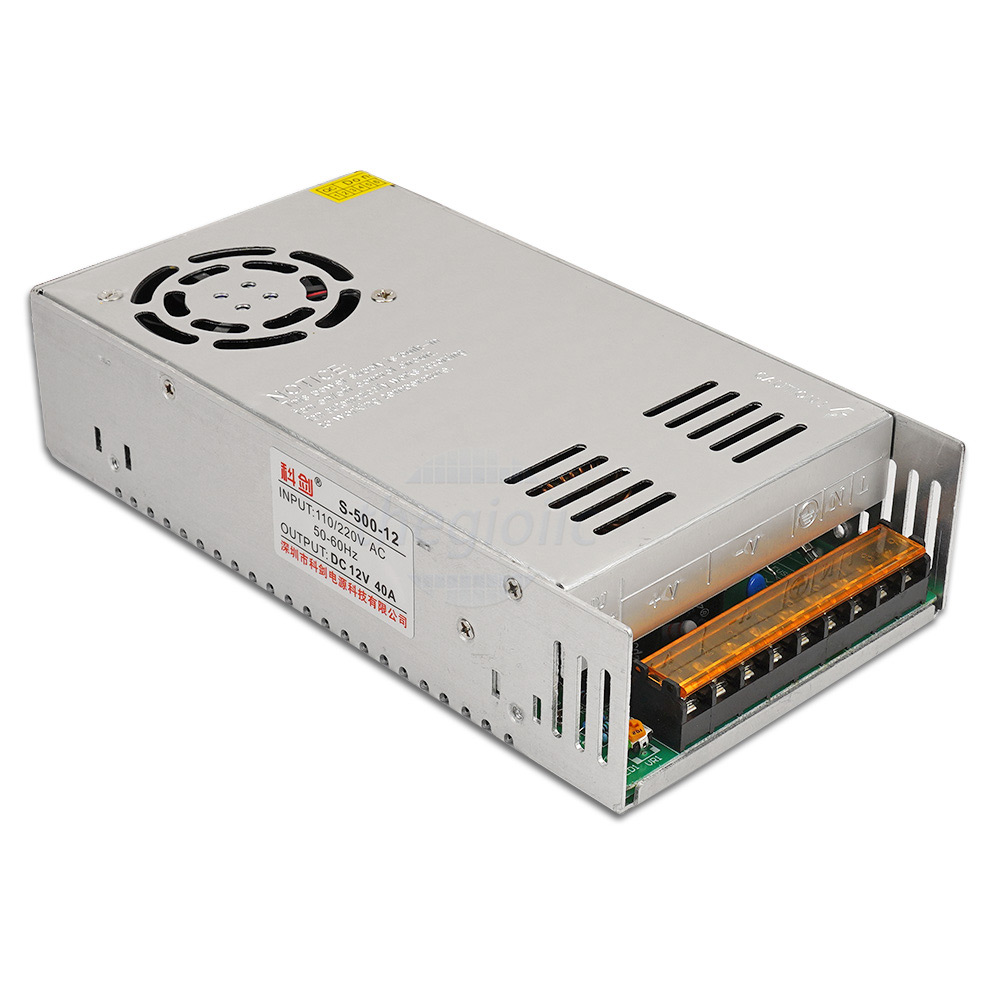
\includegraphics[width=0.6\textwidth]{img/fig35-Nguồn Xung Tổ Ong 12V 40A 480W.png} 
    \caption{Bộ nguồn xung tổ ong 12V 40A 480W}
    \label{fig35}
    \vspace{0.2cm}
\end{figure}

Việc lựa chọn nguồn xung tổ ong 12V - 40A (480W) được dựa trên tính toán dòng điện tiêu thụ của 12 động cơ servo ST3215:

Dòng điện không tải/hoạt động bình thường : Khoảng 300mA - 600mA / servo (tại 12V).
    
Dòng điện khởi động/giữ tải lớn nhất ($I_{stall}$): Khoảng 2.7A / servo (tại 12V).

Trong trường hợp xấu nhất khi robot khởi động hoặc thực hiện động tác nâng toàn thân, giả sử cả 12 servo đều chịu tải lớn, tổng dòng điện tức thời ($I_{total}$) là:

$$I_{total} = N_{servo} \times I_{stall} = 12 \times 2.7 = 32.4A$$

Theo đó, tổng công suất tiêu thụ điện tối đa ($P_{total}$) của riêng hệ thống cơ cấu chấp hành là:

$$P_{total} = I_{total} \times U = 32.4 \times 12 = 388.8W$$

Để đảm bảo an toàn và tuổi thọ cho linh kiện, tránh sụt áp nguồn khi ép tải, hệ số an toàn ($k$) thường được chọn từ 1.2 đến 1.5. Ở đây nhóm chọn hệ số $k = 1.2$, ta có yêu cầu công suất nguồn cấp tối thiểu phải đạt:

$$P_{source} \ge P_{total} \times k = 388.8 \times 1.2 = 466.56W$$

Việc lựa chọn nguồn xung tổ ong 12V - 40A (công suất cực đại 480W) là hoàn toàn chính xác và bám sát với tính toán lý thuyết ($466.56W \le 480W$). Mức công suất và dòng điện này đảm bảo khả năng đáp ứng dòng xả cao ngay cả khi robot hoạt động ở trạng thái tải nặng nhất mà không gây sụt áp hệ thống, giúp vi xử lý trung tâm Jetson Nano và các module không bị reset đột ngột.

\begin{table}[H] % <--- Chỗ này bắt buộc phải là [H]
\centering
\caption{Thông số kỹ thuật}
\renewcommand{\arraystretch}{1.3}
\begin{tabular}{ll}
\toprule
\textbf{Thuộc tính} & \textbf{Giá trị} \\
\midrule
Điện áp ngõ ra & 12V \\
Dòng điện ngõ ra & 40-49A \\
Số điện áp ra & 1 \\
Điện áp ngõ vào & 220VAC \\
Series & Khác \\
Công suất & 400-499W \\
Cách gắn & Gắn sàn \\
Vỏ bọc & Vỏ kim loại \\
\bottomrule
\end{tabular}
\end{table}

Nguồn xung tổ ong mang lại lợi thế vượt trội về độ an toàn và tính liên tục so với việc sử dụng các khối pin Li-Po trong môi trường phòng thí nghiệm. Người phát triển có thể liên tục biên dịch code, kiểm thử các quỹ đạo dáng đi hàng giờ liền mà không phải lo lắng về việc dung lượng pin cạn kiệt làm gián đoạn bài test hay sụt giảm mô-men xoắn của động cơ. Mức công suất 480W cung cấp một biên độ an toàn  dư dả để cấp nguồn song song cho cả cụm 12 servo và bo mạch xử lý trung tâm Jetson Nano (thông qua mạch giảm áp). Nhược điểm duy nhất của giải pháp này là robot bị giới hạn phạm vi di chuyển bởi chiều dài của dây cáp nguồn, khiến nó chỉ phù hợp làm mô hình thử nghiệm tại chỗ.

\subsection{Bus Servo Adapter (A)}

Các động cơ servo ST3215 được sử dụng trong thiết kế hoạt động dựa trên chuẩn giao tiếp nối tiếp bán song công (half-duplex UART). Để máy tính nhúng Jetson Nano có thể điều khiển đồng thời cả 12 động cơ này một cách an toàn và tối ưu nhất, hệ thống sử dụng hai mạch chuyển đổi tín hiệu Bus Servo Adapter (A). Mạch Adapter đóng vai trò trung gian, chuyển đổi tín hiệu UART tiêu chuẩn từ Jetson Nano (thông qua cổng USB) thành tín hiệu bus nối tiếp cấp cho các động cơ. 

Mặc dù về mặt lý thuyết, một mạch Bus Servo Adapter (A) có thể điều khiển tối đa 253 động cơ nối tiếp, nhưng trong thực tế, dòng điện khởi động của 12 động cơ ST3215 có thể lên đến 32.4A. Việc sử dụng song song hai mạch Adapter mang lại những lợi ích thiết thực:
\begin{itemize}
    \item \textbf{Phân tán dòng điện:} Mỗi mạch Adapter chỉ cần chịu tải dòng điện cho 6 động cơ (khoảng 16.2A tối đa), giảm thiểu đáng kể rủi ro quá tải nhiệt và cháy nổ cho bản mạch in (PCB) của Adapter so với việc gánh toàn bộ tải.
    \item \textbf{Tối ưu hóa đi dây:} Phân chia hệ thống thành hai cụm (ví dụ: nửa trái và nửa phải của robot), giúp sơ đồ đi dây trở nên gọn gàng, logic và dễ dàng kiểm tra, bảo trì hơn.
\end{itemize}

Thông qua các giao thức truyền thông và tập lệnh được định nghĩa sẵn, hệ thống có thể điều khiển hiệu quả các biến số như: góc quay, tốc độ di chuyển, giới hạn tải, cũng như đọc các tín hiệu phản hồi về nhiệt độ, điện áp và vị trí thực tế của từng động cơ.

\begin{figure}[H]
    \centering
    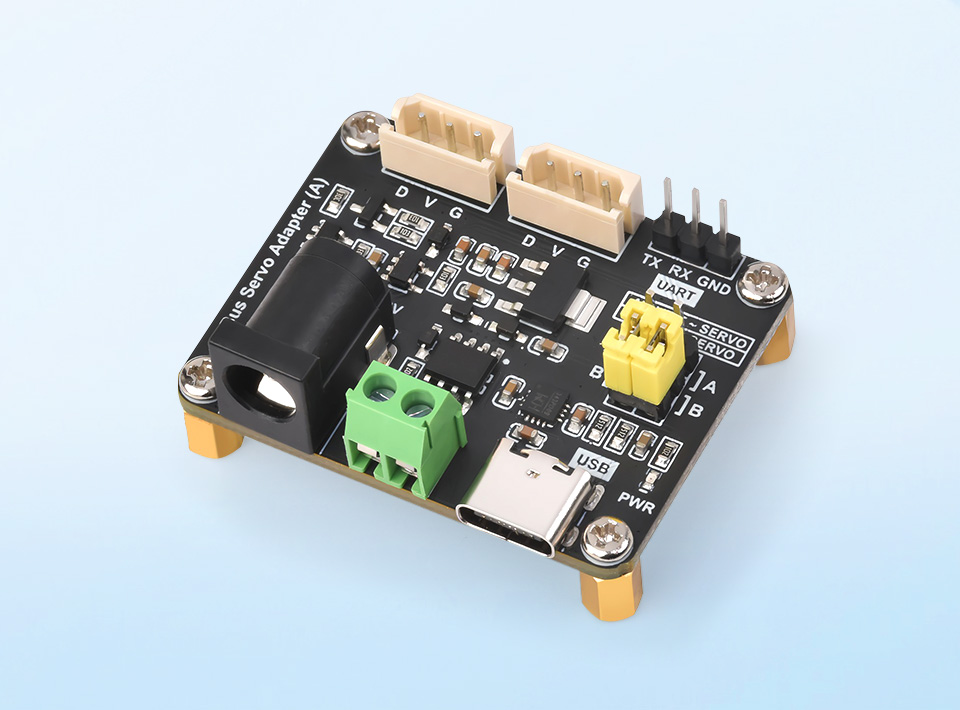
\includegraphics[width=0.6\textwidth]{img/fig36-Bus-Servo-Adapter-A-details-1.jpg} 
    \caption{Bus Servo Adapter (A)}
    \label{fig36}
    \vspace{0.2cm}
\end{figure}

\begin{table}[H]
    \centering
    \caption{Thông số kỹ thuật mạch Bus Servo Adapter (A)}
    \label{tab:adapter_specs}
    \renewcommand{\arraystretch}{1.5} % Tăng độ rộng giữa các hàng cho thoáng và đẹp giống ảnh
    \begin{tabular}{ll}
        \hline
        \textbf{Power Supply} & DC 9 $\sim$ 12.6V (ST series servo) \\ \hline
        \textbf{Power supply connector} & 5.5 $\times$ 2.1mm DC \\ \hline
        \textbf{communication interface} & UART \\ \hline
        \textbf{Dimensions} & 42.00 $\times$ 33.00mm \\ \hline
        \textbf{Mounting hole size} & 2.50mm \\ \hline
        \textbf{Mounting hole spacing} & 37.00 $\times$ 28.00mm \\ \hline
    \end{tabular}
\end{table}

\subsection{Bộ đo lường quán tính }

Module IMU (Inertial Measurement Unit) đóng vai trò cốt lõi trong hệ thống phản hồi thăng bằng của robot. Thay vì sử dụng các cảm biến quán tính thô, đồ án này ứng dụng module GY-BNO055 \cite{bno055} --- một board mạch breakout nhỏ gọn được thiết kế trên nền tảng chip cảm biến BNO055 của Bosch Sensortec. Module tích hợp sẵn gia tốc kế 3 trục, con quay hồi chuyển 3 trục, từ kế 3 trục và đặc biệt là một vi xử lý ARM Cortex-M0+ 32-bit chạy thuật toán kết hợp cảm biến (Sensor Fusion) độc quyền của Bosch, cho phép xuất trực tiếp dữ liệu định hướng tuyệt đối mà không cần bộ lọc ngoại vi.

\begin{figure}[H]
\centering

\includegraphics[width=0.55\textwidth]{img/fig37-IMU-BNO055.png}
\caption{Module cảm biến 9 trục thông minh GY-BNO055 (mặt trước và mặt sau)}
\label{fig37}
\vspace{0.2cm}
\end{figure}

Module GY-BNO055 sở hữu kích thước cực kỳ nhỏ gọn (20,9~mm $\times$ 11,9~mm), rất phù hợp để gắn trực tiếp lên khung thân robot mà không chiếm nhiều không gian. Board mạch được bố trí 8 chân tín hiệu gồm: VIN (nguồn cấp), GND (mass), SCL/Rx (xung nhịp I2C hoặc nhận UART), SDA/Tx (dữ liệu I2C hoặc phát UART), ADD (chọn địa chỉ I2C), INT (ngắt ngoài), BOOT (chế độ nạp firmware) và RESET (khởi động lại phần cứng). Mạch tích hợp sẵn bộ ổn áp nội cho phép cấp nguồn linh hoạt từ 3,3V đến 5V qua chân VIN.

Về mặt kiến trúc phần cứng, nhóm đã tối ưu hóa hệ thống bằng cách loại bỏ hoàn toàn vi điều khiển trung gian như cấu trúc dùng STM32. Nền tảng phát triển giờ đây được triển khai trực tiếp trên môi trường hệ điều hành Linux của Jetson Nano. Cảm biến BNO055 được kết nối và giao tiếp thẳng với Jetson Nano thông qua bus I2C (sử dụng hai chân SCL và SDA). Việc lập trình thu thập dữ liệu được thực hiện bằng ngôn ngữ Python. Sự thay đổi này không chỉ giúp giảm thiểu đáng kể độ trễ truyền dữ liệu mà còn tối giản hóa độ phức tạp của việc đi dây phần cứng.

Khác với các cảm biến truyền thống (như MPU6050) dễ bị nhiễu từ môi trường và đòi hỏi người lập trình phải tự xây dựng các bộ lọc toán học phức tạp (như Complementary Filter hay Kalman Filter) trên máy tính chủ, BNO055 xử lý toàn bộ khối lượng công việc này ở cấp độ phần cứng nội bộ. Tính năng Sensor Fusion của BNO055 tự động tính toán và xuất trực tiếp dữ liệu định hướng dưới dạng các góc Euler (Roll, Pitch, Yaw) hoặc Quaternion với độ chính xác cao và tần số cập nhật nhanh. Do đó, bài toán của nhóm được chuyển từ việc ``viết bộ lọc nhiễu'' sang việc quản lý quy trình tự hiệu chuẩn của cảm biến.
\begin{table}[H]
\centering
\caption{Thông số kỹ thuật module cảm biến GY-BNO055}
\label{tab:bno055_specs}
\renewcommand{\arraystretch}{1.3}
\begin{tabular}{ll}
\toprule
\textbf{Thông số} & \textbf{Giá trị} \\
\midrule
Chip cảm biến & Bosch BNO055 (SiP -- System in Package) \\
Số trục đo & 9 trục (Accelerometer + Gyroscope + Magnetometer) \\
Điện áp hoạt động & 3.3V -- 5V (qua chân VIN, tích hợp bộ ổn áp nội) \\
Chuẩn giao tiếp & I2C / UART (chọn qua chân BOOT) \\
Địa chỉ I2C mặc định & 0x28 (chân ADD = LOW); 0x29 (chân ADD = HIGH) \\
Gia tốc kế (Accelerometer) & $\pm$2g / $\pm$4g / $\pm$8g / $\pm$16g \\
Con quay hồi chuyển (Gyroscope) & $\pm$125$^\circ$/s đến $\pm$2000$^\circ$/s \\
Từ kế (Magnetometer) & $\pm$1300$\mu$T (trục x,y); $\pm$2500$\mu$T (trục z) \\
Bộ xử lý tích hợp & ARM Cortex-M0+ (chạy thuật toán Sensor Fusion) \\
Dữ liệu đầu ra & Quaternion, góc Euler, vector trọng lực, gia tốc tuyến tính \\
Tần số cập nhật Fusion & Lên đến 100 Hz \\
Kích thước mạch & 20,9 $\times$ 11,9 mm \\
Số chân tín hiệu & 8 (VIN, GND, SCL/Rx, SDA/Tx, ADD, INT, BOOT, RESET) \\
Nhiệt độ hoạt động & $-40^\circ$C đến $+85^\circ$C \\
\bottomrule
\end{tabular}
\end{table}
\subsection{Mạch Giảm Áp }

Bên cạnh nguồn năng lượng 12V cung cấp trực tiếp cho hệ thống động cơ servo, thiết bị xử lý trung tâm là máy tính nhúng Jetson Nano Developer Kit B01 yêu cầu một nguồn điện DC 5V ổn định để hoạt động. Trong các điều kiện tải nặng, chẳng hạn như khi tính toán động học nghịch liên tục cho 12 bậc tự do hoặc xử lý thuật toán cân bằng, Jetson Nano có thể tiêu thụ dòng điện lên đến 4A. Việc sử dụng các IC ổn áp tuyến tính thông thường sẽ gây ra hiện tượng hao phí nhiệt lượng rất lớn và không đáp ứng đủ dòng tải yêu cầu.

Do đó, mạch giảm áp xung\textbf{XL4015 5A 75W} đã được lựa chọn để thực hiện nhiệm vụ chuyển đổi điện áp từ 12V của nguồn tổ ong xuống mức 5V an toàn cho Jetson Nano. Ưu điểm nổi bật của XL4015 là hiệu suất chuyển đổi năng lượng cao (lên đến 96\%), tần số băm xung 180KHz giúp giảm thiểu gợn điện áp, và khả năng cấp dòng đầu ra tối đa lên tới 5A. Điều này tạo ra một biên độ dự trữ công suất an toàn, giúp máy tính nhúng không bị sụt áp đột ngột dẫn đến tắt nguồn trong quá trình vận hành. Hơn nữa, mạch còn được tích hợp các tính năng bảo vệ ngắn mạch và bảo vệ quá nhiệt, đảm bảo an toàn tối đa cho các bo mạch điện tử đắt tiền phía sau.

\begin{figure}[H]
    \centering
    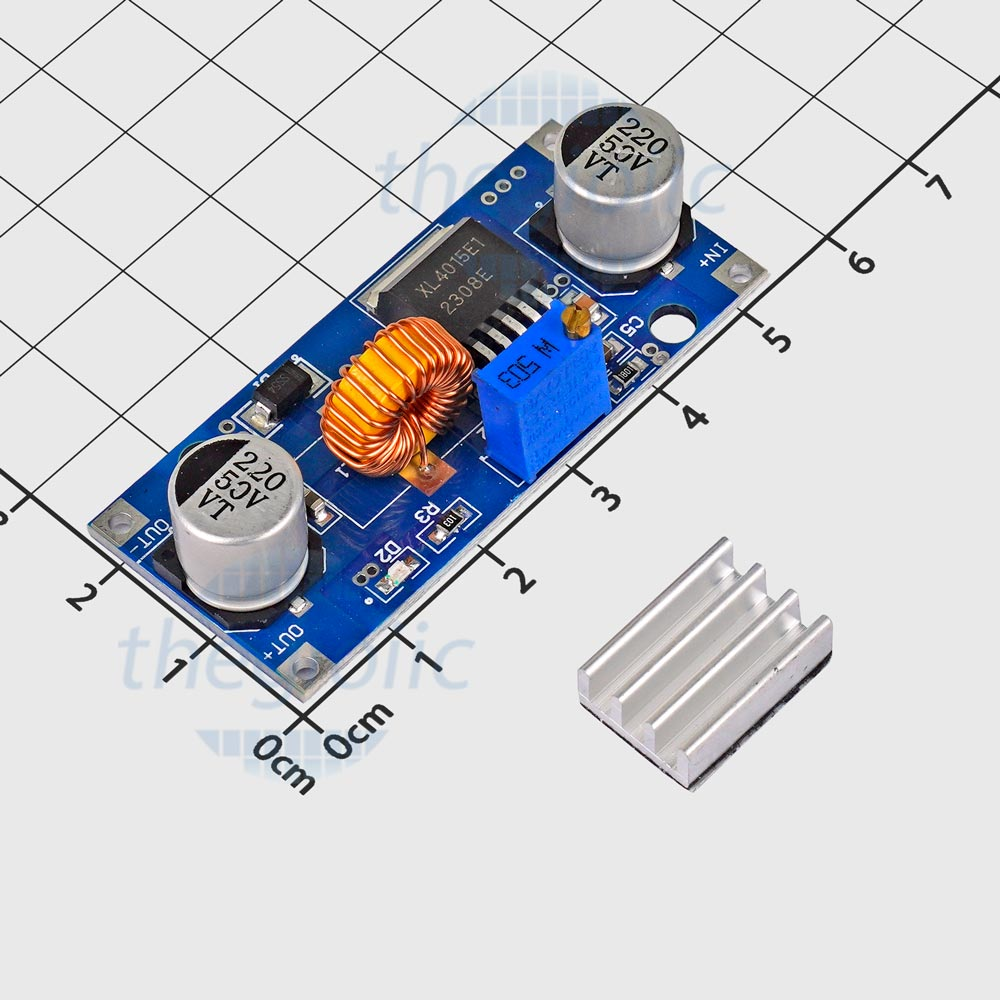
\includegraphics[width=0.6\textwidth]{img/fig38-Mạch giảm áp.jpg} 
    \caption{Mạch giảm áp XL4015 5A 75W}
    \label{fig38}
    \vspace{0.2cm}
\end{figure}

Các thông số kỹ thuật chi tiết của mạch giảm áp XL4015 được trình bày cụ thể trong Bảng \ref{tab:xl4015_specs}. Mức điện áp ngõ ra đã được nhóm tác giả tinh chỉnh qua biến trở tích hợp trên mạch để đạt chính xác mức 5.0V - 5.1V nhằm bù trừ sụt áp trên dây dẫn trước khi cấp vào Jetson Nano.

\begin{table}[H]
    \centering
    \caption{Thông số kỹ thuật mạch giảm áp XL4015 5A 75W}
    \label{tab:xl4015_specs}
    \renewcommand{\arraystretch}{1.5} 
    \begin{tabular}{ll}
        \hline
        \textbf{Điện áp ngõ vào} & 5 $\sim$ 32 VDC \\ \hline
        \textbf{Điện áp ngõ ra} & 1.25 $\sim$ 30 VDC (Tinh chỉnh về 5V cấp cho vi xử lý) \\ \hline
        \textbf{Dòng ngõ ra} & 0 $\sim$ 5A \\ \hline
        \textbf{Công suất ngõ ra} & 75W \\ \hline
        \textbf{Nhiệt độ làm việc} & -40 $\sim$ +85$^\circ$C \\ \hline
        \textbf{Tần số hoạt động} & 180KHz \\ \hline
        \textbf{Hiệu suất tối đa} & 96\% \\ \hline
        \textbf{Bảo vệ ngắn mạch} & Có (giới hạn 8A) \\ \hline
        \textbf{Bảo vệ quá nhiệt} & Có \\ \hline
    \end{tabular}
\end{table}


\subsection{Cơ cấu chấp hành: Động cơ Bus Servo ST3215}

Việc lựa chọn cơ cấu chấp hành có ảnh hưởng trực tiếp đến hiệu năng di chuyển, khả năng giữ thăng bằng và độ phức tạp của hệ thống phần cứng robot bốn chân. Trong đồ án này, động cơ Bus Servo ST3215 và phiên bản tốc độ cao ST3215-HS \cite{waveshare_st3215} đã được lựa chọn làm thiết bị truyền động cho toàn bộ 12 bậc tự do của robot. 

Để làm rõ tính ưu việt và lý do lựa chọn công nghệ truyền động này cho mô hình nguyên mẫu, nhóm đã tiến hành đánh giá và so sánh dòng động cơ Bus Servo nối tiếp với hai loại cơ cấu chấp hành phổ biến khác: Động cơ Servo điều khiển bằng xung PWM truyền thống và Động cơ không chổi than (BLDC).

\begin{table}[H]
\centering
\caption{Bảng so sánh các loại cơ cấu chấp hành áp dụng cho Robot bốn chân}
\label{tab:motor_comparison}
\renewcommand{\arraystretch}{1.3}
\begin{tabular}{|p{0.2\linewidth}|p{0.2\linewidth}|p{0.2\linewidth}|p{0.25\linewidth}|}
\hline
\textbf{Tiêu chí} & \textbf{Động cơ Servo PWM truyền thống} & \textbf{Động cơ BLDC (Tích hợp Driver)} & \textbf{Động cơ Bus Servo nối tiếp} \\ \hline
\textbf{Giao thức điều khiển} & Xung PWM (Đơn hướng) & CAN / RS485 (Song công) & UART bán song công (Half-duplex) \\ \hline
\textbf{Hệ thống dây dẫn} & Rất phức tạp (Mỗi motor 1 dây tín hiệu riêng) & Tối giản (Nối tiếp chuỗi - Daisy chain) & Tối giản (Nối tiếp chuỗi - Daisy chain) \\ \hline
\textbf{Khả năng phản hồi (Feedback)} & Không có & Vị trí, tốc độ, dòng điện, nhiệt độ (FOC) & Vị trí thực tế, tốc độ, tải, nhiệt độ, điện áp \\ \hline
\textbf{Mô-men xoắn} & Thường ở mức thấp đến trung bình & Rất cao & Cao (Tối ưu trong tầm giá) \\ \hline
\textbf{Khối lượng \& Kích thước} & Nhẹ & Nặng, cồng kềnh & Gọn nhẹ \\ \hline
\textbf{Giá thành} & Rất thấp & Rất cao & Trung bình - Hợp lý \\ \hline
\textbf{Độ phù hợp} & Thấp (Do không có phản hồi và thiếu lực) & Thấp (Dư thừa công suất, chi phí quá cao) & \textbf{Rất cao (Đạt điểm cân bằng tối ưu)} \\ \hline
\end{tabular}
\end{table}

Sau khi xác định kiến trúc truyền động tối ưu là sử dụng \textbf{Bus Servo nối tiếp} thay vì Servo PWM hay động cơ BLDC, nhóm đã tiến hành khảo sát và đánh giá các dòng Bus Servo phổ biến trên thị trường để tìm ra phương án phù hợp nhất cho hệ thống 12 bậc tự do của robot.

Ba đại diện tiêu biểu được đưa ra so sánh bao gồm: Hiwonder LX-16A, Waveshare ST3215 và Dynamixel XL430-W250-T.

\begin{table}[H]
\centering
\caption{So sánh các dòng Bus Servo nối tiếp phổ biến trên thị trường}
\label{tab:bus_servo_comparison}
\renewcommand{\arraystretch}{1.3}
\begin{tabular}{|p{0.2\linewidth}|p{0.2\linewidth}|p{0.25\linewidth}|p{0.2\linewidth}|}
\hline
\textbf{Tiêu chí} & \textbf{Hiwonder LX-16A} & \textbf{Waveshare ST3215 (Được chọn)} & \textbf{Dynamixel XL430-W250-T} \\ \hline
\textbf{Giao thức} & TTL UART (Half-duplex) & TTL UART (Half-duplex) & TTL UART (Half-duplex) \\ \hline
\textbf{Điện áp} & 6.0V - 8.4V (Tối ưu 7.4V) & 6.0V - 12.6V (Tối ưu 12V) & 10.0V - 14.8V (Tối ưu 11.1V) \\ \hline
\textbf{Lực xoắn tối đa} & 17 kg.cm (@7.4V) & 30 kg.cm / 20 kg.cm (@12V) & $\sim$15.3 kg.cm (1.5 N.m @11.1V) \\ \hline
\textbf{Cảm biến vị trí} & Biến trở (Potentiometer) & Từ tính (Magnetic Encoder $360^{\circ}$) & Từ tính (Absolute Encoder) \\ \hline
\textbf{Độ phân giải góc} & 0.24$^{\circ}$ & 0.088$^{\circ}$ & 0.088$^{\circ}$ \\ \hline
\textbf{Tốc độ truyền} & 115200 bps & Lên đến 1 Mbps & Lên đến 4.5 Mbps \\ \hline
\textbf{Bộ điều khiển} & Cơ bản (P) & Nâng cao (PI) & Cao cấp (PID vị trí, vận tốc, dòng) \\ \hline
\textbf{Giá thành} & Thấp ($\sim$300.000 VNĐ) & Trung bình ($\sim$500.000 VNĐ) & Rất cao ($\sim$1.500.000 VNĐ) \\ \hline
\end{tabular}
\end{table}

Dựa trên các thông số phân tích từ Bảng \ref{tab:bus_servo_comparison}, Waveshare ST3215 được lựa chọn là giải pháp tối ưu nhất cho hệ thống cơ cấu chấp hành của đồ án vì những lý do sau:

\begin{itemize}
    \item \textbf{Khắc phục nhược điểm của LX-16A:} Mặc dù Hiwonder LX-16A có lợi thế về giá thành thấp, nhưng lực xoắn tối đa chỉ đạt 17 kg.cm, không đủ để đáp ứng tải trọng động khi robot di chuyển hoặc thực hiện các tư thế phức tạp. Hơn nữa, việc sử dụng biến trở (Potentiometer) làm cảm biến vị trí khiến độ phân giải góc thấp ($0.24^{\circ}$) và dễ bị hao mòn cơ học theo thời gian. Bộ điều khiển của LX-16A chỉ dừng ở mức cơ bản (P), dẫn đến sai số tĩnh lớn và khả năng bám quỹ đạo kém.
    \item \textbf{Cân bằng hiệu năng và chi phí so với Dynamixel:} Dòng Dynamixel XL430-W250-T sở hữu bộ điều khiển PID hoàn chỉnh cùng nhiều tính năng cao cấp. Tuy nhiên, mức giá cực kỳ đắt đỏ (gấp khoảng 3 lần ST3215). Với yêu cầu 12 bậc tự do, việc sử dụng Dynamixel sẽ làm chi phí phần cứng vượt quá ngân sách cho phép. Thêm vào đó, lực xoắn của XL430-W250-T ($\sim$15.3 kg.cm) lại thấp hơn ST3215, đòi hỏi phải sử dụng cơ cấu truyền động phức tạp để khuyếch đại lực.
    \item \textbf{Ưu điểm vượt trội của ST3215:} Waveshare ST3215 mang lại điểm cân bằng hoàn hảo giữa hiệu năng cơ học và chi phí. Lực xoắn cao (lên đến 30 kg.cm ở 12V) cung cấp dư dả công suất để robot duy trì thăng bằng và thực hiện dáng đi. Cảm biến vị trí từ tính (Magnetic Encoder $360^{\circ}$) với độ phân giải rất cao ($0.088^{\circ}$) cung cấp phản hồi góc chính xác tuyệt đối mà không lo bị hao mòn. Tốc độ truyền tải 1 Mbps hoàn toàn đáp ứng được yêu cầu của vòng lặp điều khiển thời gian thực. Đặc biệt, bộ điều khiển PI tích hợp sẵn giúp động cơ khử sai số tĩnh, đảm bảo robot bám sát quỹ đạo dáng đi một cách mượt mà và ổn định.
\end{itemize}

\subsection{Hệ thống Phân phối Năng lượng và Lựa chọn Dây dẫn}

Để đảm bảo hệ thống 12 động cơ hoạt động ổn định ở dòng tải cao mà không bị sụt áp, việc thiết kế sơ đồ đi dây và lựa chọn tiết diện dây dẫn đóng vai trò cực kỳ quan trọng. Dựa trên phân tích dòng điện tổng ($I_{total} \approx 32.4A$) từ nguồn tổ ong, hệ thống dây dẫn được chia thành 3 cấp độ với các tiêu chuẩn AWG (American Wire Gauge) khác nhau, được phân phối qua các khối đầu nối nguồn (Terminal Block).

\begin{figure}[H]
    \centering
    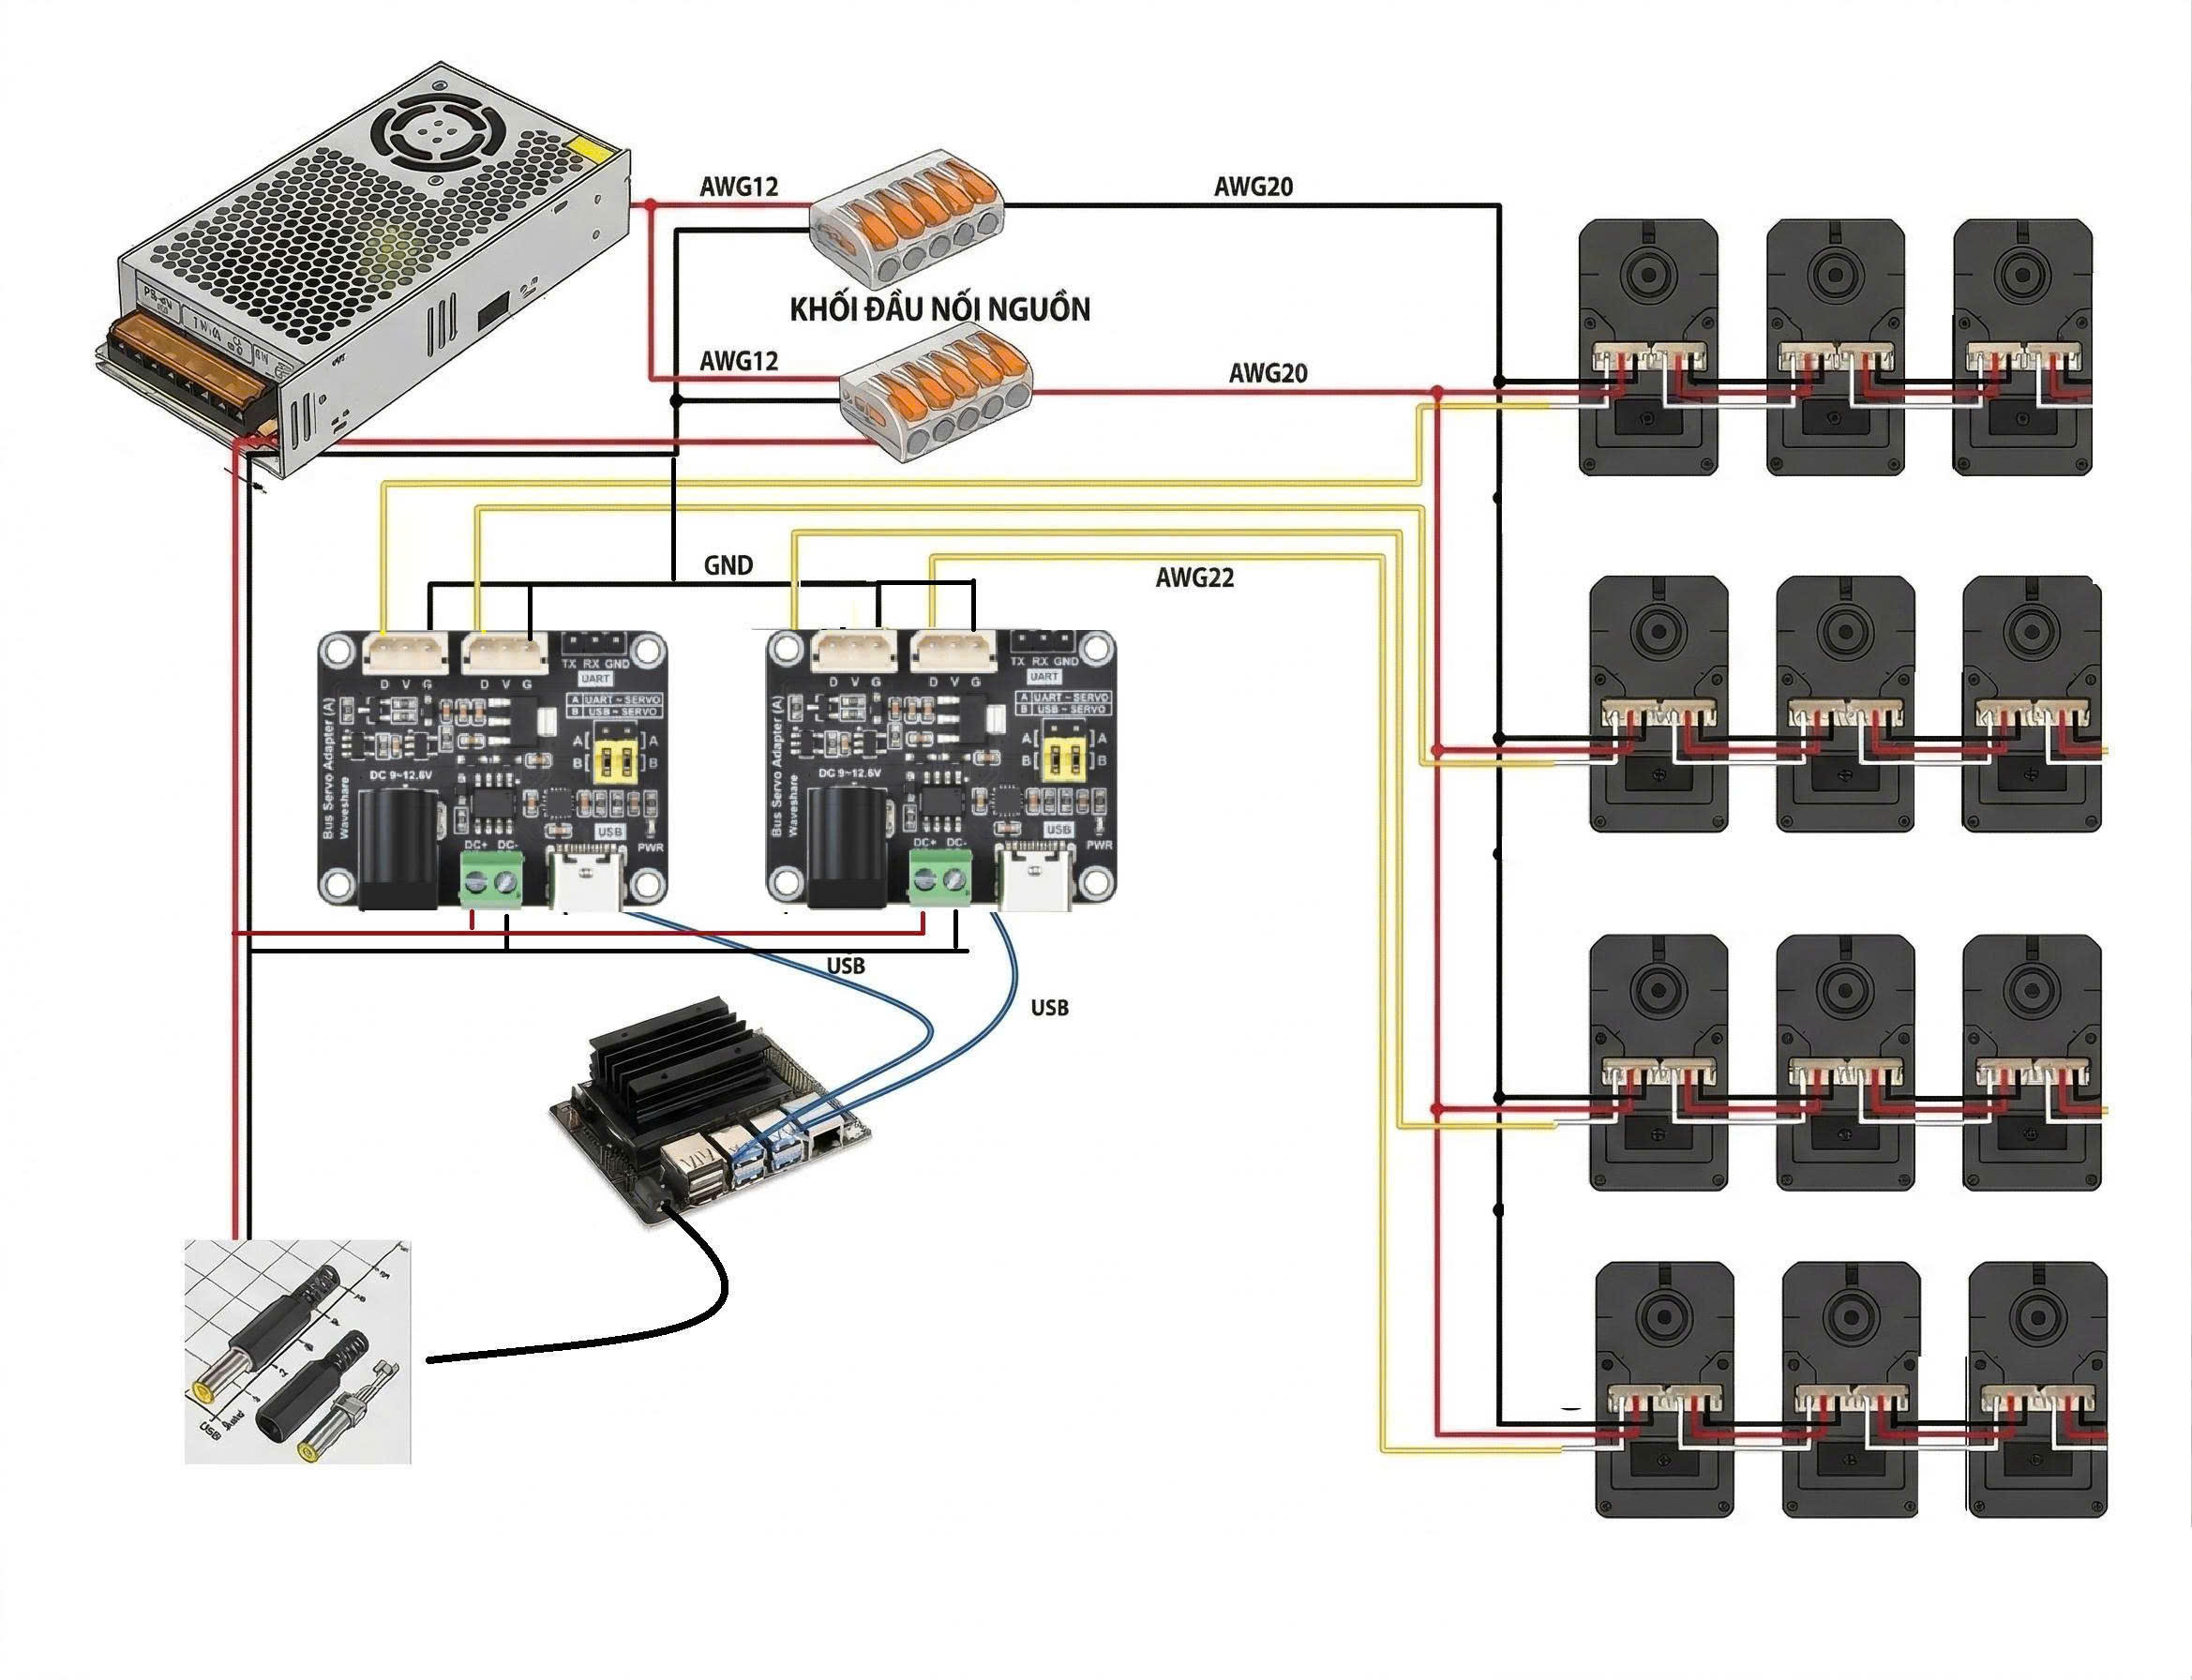
\includegraphics[width=1.0\textwidth]{img/fig44-sododiday-hethong.jpg} 
    \caption{Sơ đồ phân phối điện áp và tín hiệu tổng thể của robot}
    \label{fig44}
    \vspace{0.2cm}
\end{figure}

Dựa trên thông số kỹ thuật (Datasheet) của các loại dây lõi đồng, nhóm đã đưa ra thiết kế đi dây như sau:

\textbf{1. Trục nguồn chính (Từ Nguồn tổ ong đến Khối đấu nối): Dây AWG 12}
\begin{itemize}
    \item \textbf{Chức năng:} Truyền tải toàn bộ dòng điện từ nguồn xung 12V-40A đến các khối chia nguồn trung tâm.
    \item \textbf{Thông số kỹ thuật (AWG 12):} Đường kính lõi khoảng 2.05 mm, tiết diện 3.31 mm$^2$. Khả năng chịu dòng (Ampacity) trong điều kiện không khí mở có thể lên đến 30A - 40A, với điện trở cực kỳ thấp (khoảng 5.2 $\Omega$/km).
    \item \textbf{Lý do lựa chọn:} Trục chính phải gánh toàn bộ tải của 12 servo cùng lúc (dòng xả tức thời có thể đạt 32.4A). Dây AWG 12 hoàn toàn đáp ứng được mức dòng điện này mà không sinh nhiệt hay gây sụt áp đáng kể trên đường truyền.
\end{itemize}

\textbf{2. Nhánh nguồn phụ (Từ Khối đấu nối đến Servo đầu tiên): Dây AWG 20}
\begin{itemize}
    \item \textbf{Chức năng:} Cấp nguồn trực tiếp từ khối chia nguồn đến động cơ Servo đầu tiên của mỗi nhánh (chuỗi 3 servo cho mỗi chân).
    \item \textbf{Thông số kỹ thuật (AWG 20):} Đường kính lõi 0.81 mm, tiết diện 0.52 mm$^2$. Khả năng chịu dòng định mức khoảng 5A (tối đa có thể lên 11A tùy lớp cách điện).
    \item \textbf{Lý do lựa chọn:} Mỗi nhánh chân gồm 3 servo ST3215, với dòng khởi động tổng cộng khoảng 8.1A. Dây AWG 20 cung cấp sự cân bằng hoàn hảo giữa khả năng chịu tải và độ linh hoạt (mềm dẻo) để luồn lách qua các khớp cơ khí của robot.
\end{itemize}

\textbf{3. Bus tín hiệu truyền thông (Từ Adapter đến Servo): Dây AWG 22}
\begin{itemize}
    \item \textbf{Chức năng:} Truyền tín hiệu UART (Data) từ mạch Bus Servo Adapter đến các servo, và kết nối chung chân Mass (GND) để đồng bộ mức điện áp logic.
    \item \textbf{Thông số kỹ thuật (AWG 22):} Đường kính lõi 0.64 mm, tiết diện 0.326 mm$^2$. 
    \item \textbf{Lý do lựa chọn:} Đường truyền dữ liệu không mang dòng điện tải cao (chỉ vài mA). Việc sử dụng dây AWG 22 giúp cáp tín hiệu nhỏ gọn, hạn chế nhiễu chéo, dễ dàng bấm cos và đi dây nối tiếp (daisy-chain) qua từng servo mà không gây cản trở chuyển động của các khớp.
\end{itemize}

Việc thiết kế phân nhánh nguồn thông qua Terminal Block kết hợp với việc tính toán và lựa chọn đúng cỡ dây AWG từ datasheet giúp giải quyết triệt để vấn đề sụt áp trên đường dây (Voltage Drop), đảm bảo 12 động cơ ở cuối chuỗi vẫn nhận đủ điện áp 12V để sinh ra mô-men xoắn tối đa.

\section{Các Giao thức Truyền thông của Hệ thống}

Toàn bộ hệ thống điều khiển sử dụng hai giao thức truyền thông chính: I2C để thu thập dữ liệu cảm biến và UART để điều khiển cơ cấu chấp hành. Vi xử lý trung tâm Jetson Nano đóng vai trò là thiết bị chủ , liên tục nhận dữ liệu tư thế không gian từ module IMU và thực hiện các tính toán động học nghịch dựa trên thông số hình học của các chân. Để hoàn thành nhiệm vụ này, việc đầu tiên nhóm thực hiện là thiết lập giao tiếp I2C giữa Jetson Nano và cảm biến IMU. Đây là một bước có thể thực hiện hiệu quả thông qua môi trường lập trình Python trên hệ điều hành Linux (Ubuntu), bằng cách khai báo đúng địa chỉ phần cứng và sử dụng trực tiếp các chân bus I2C tích hợp sẵn trên bo mạch Jetson.

\begin{figure}[H]
    \centering
    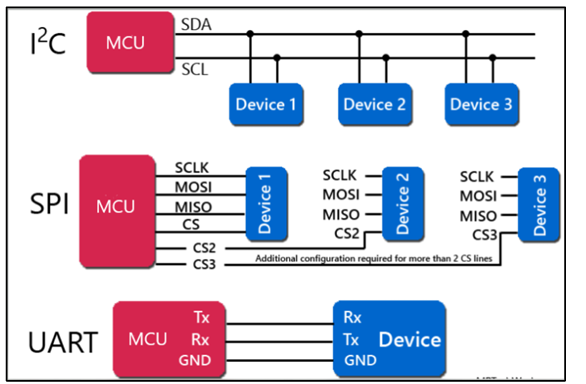
\includegraphics[width=0.6\textwidth]{img/fig39-Different Communication Protocols .png} 
    \caption{Các giao thức truyền thông khác nhau}
    \label{fig39}
    \vspace{0.2cm}
    \textit{}
\end{figure}

Phần công việc đòi hỏi nhiều sự tinh chỉnh và thời gian hoàn thành hơn là việc thiết lập và tối ưu hóa đường truyền tín hiệu xuống các động cơ servo. Để điều khiển đồng bộ 12 động cơ ST3215, hệ thống sử dụng chuẩn giao tiếp UART (thông qua hai cổng USB) kết nối với hai mạch Bus Servo Adapter (A). Các mạch Adapter này hoạt động ở tốc độ truyền tải (baudrate) lên đến 1 Mbps, làm nhiệm vụ phân phối các gói tin lệnh dạng nối tiếp đến từng địa chỉ định danh (ID) của động cơ trên cùng một đường bus truyền tín hiệu tương ứng. Việc chuyển đổi từ tín hiệu mức logic của Jetson Nano sang chuẩn bus nối tiếp bán song công, kết hợp với việc chia thành 2 bus riêng biệt, giúp đơn giản hóa đáng kể sơ đồ đi dây vật lý mà vẫn đảm bảo tốc độ phản hồi siêu tốc độ theo thời gian thực cho vòng lặp điều khiển PID.

\begin{figure}[H]
    \centering
    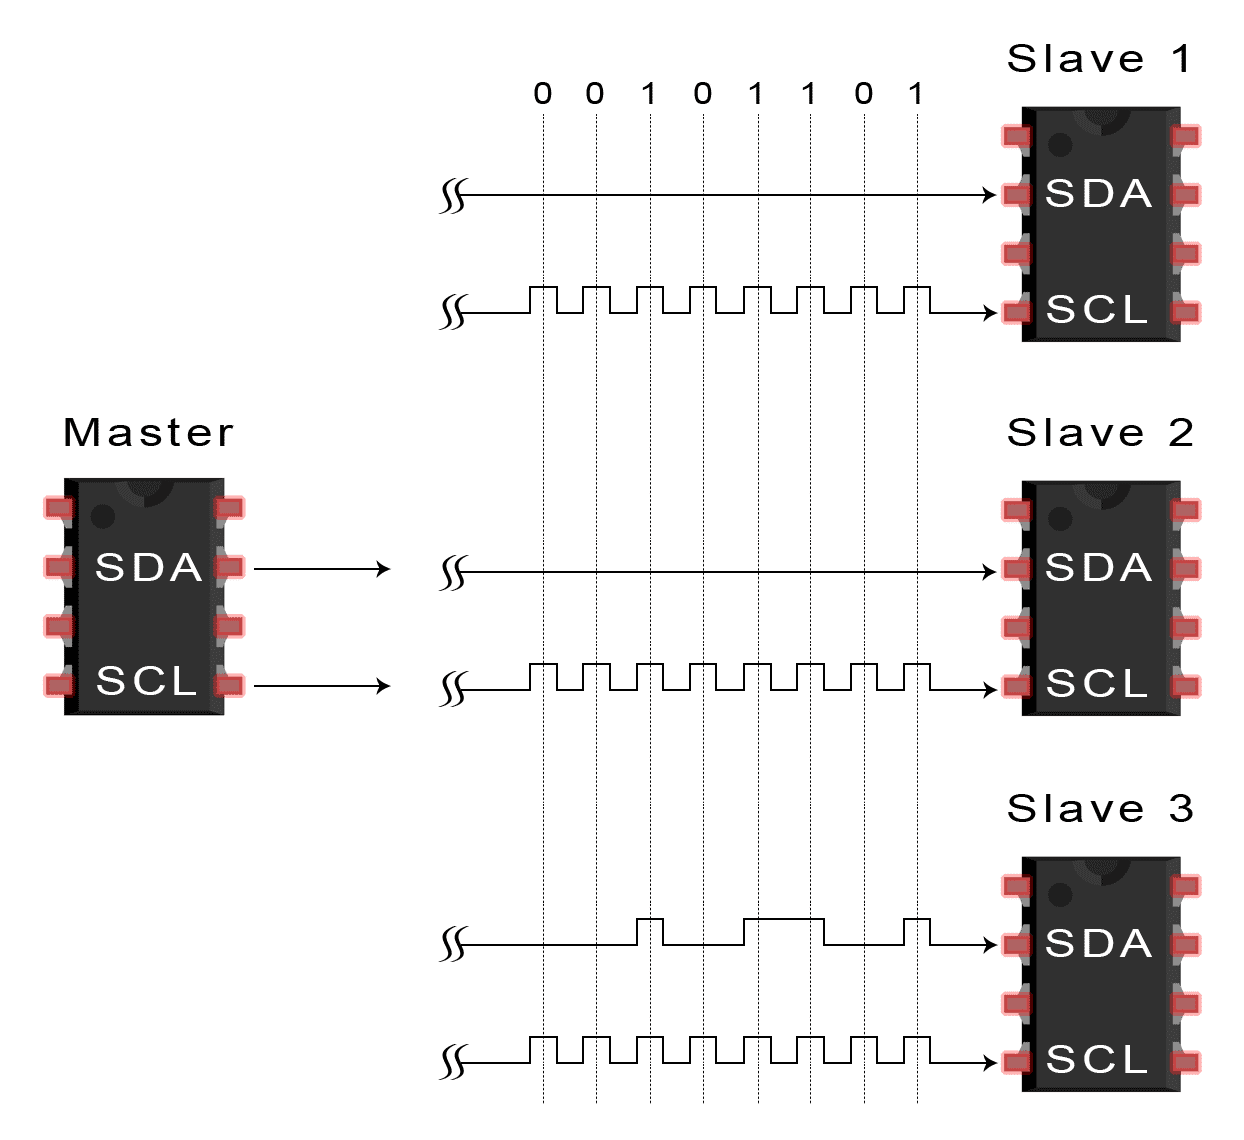
\includegraphics[width=0.6\textwidth]{img/fig40-Introduction-to-I2C-Data-Transmission-Diagram-Data-Frame.png} 
    \caption{Giao thức truyền thông I2C}
    \label{fig40}
    \vspace{0.2cm}
\end{figure}
\begin{figure}[H]
    \centering
    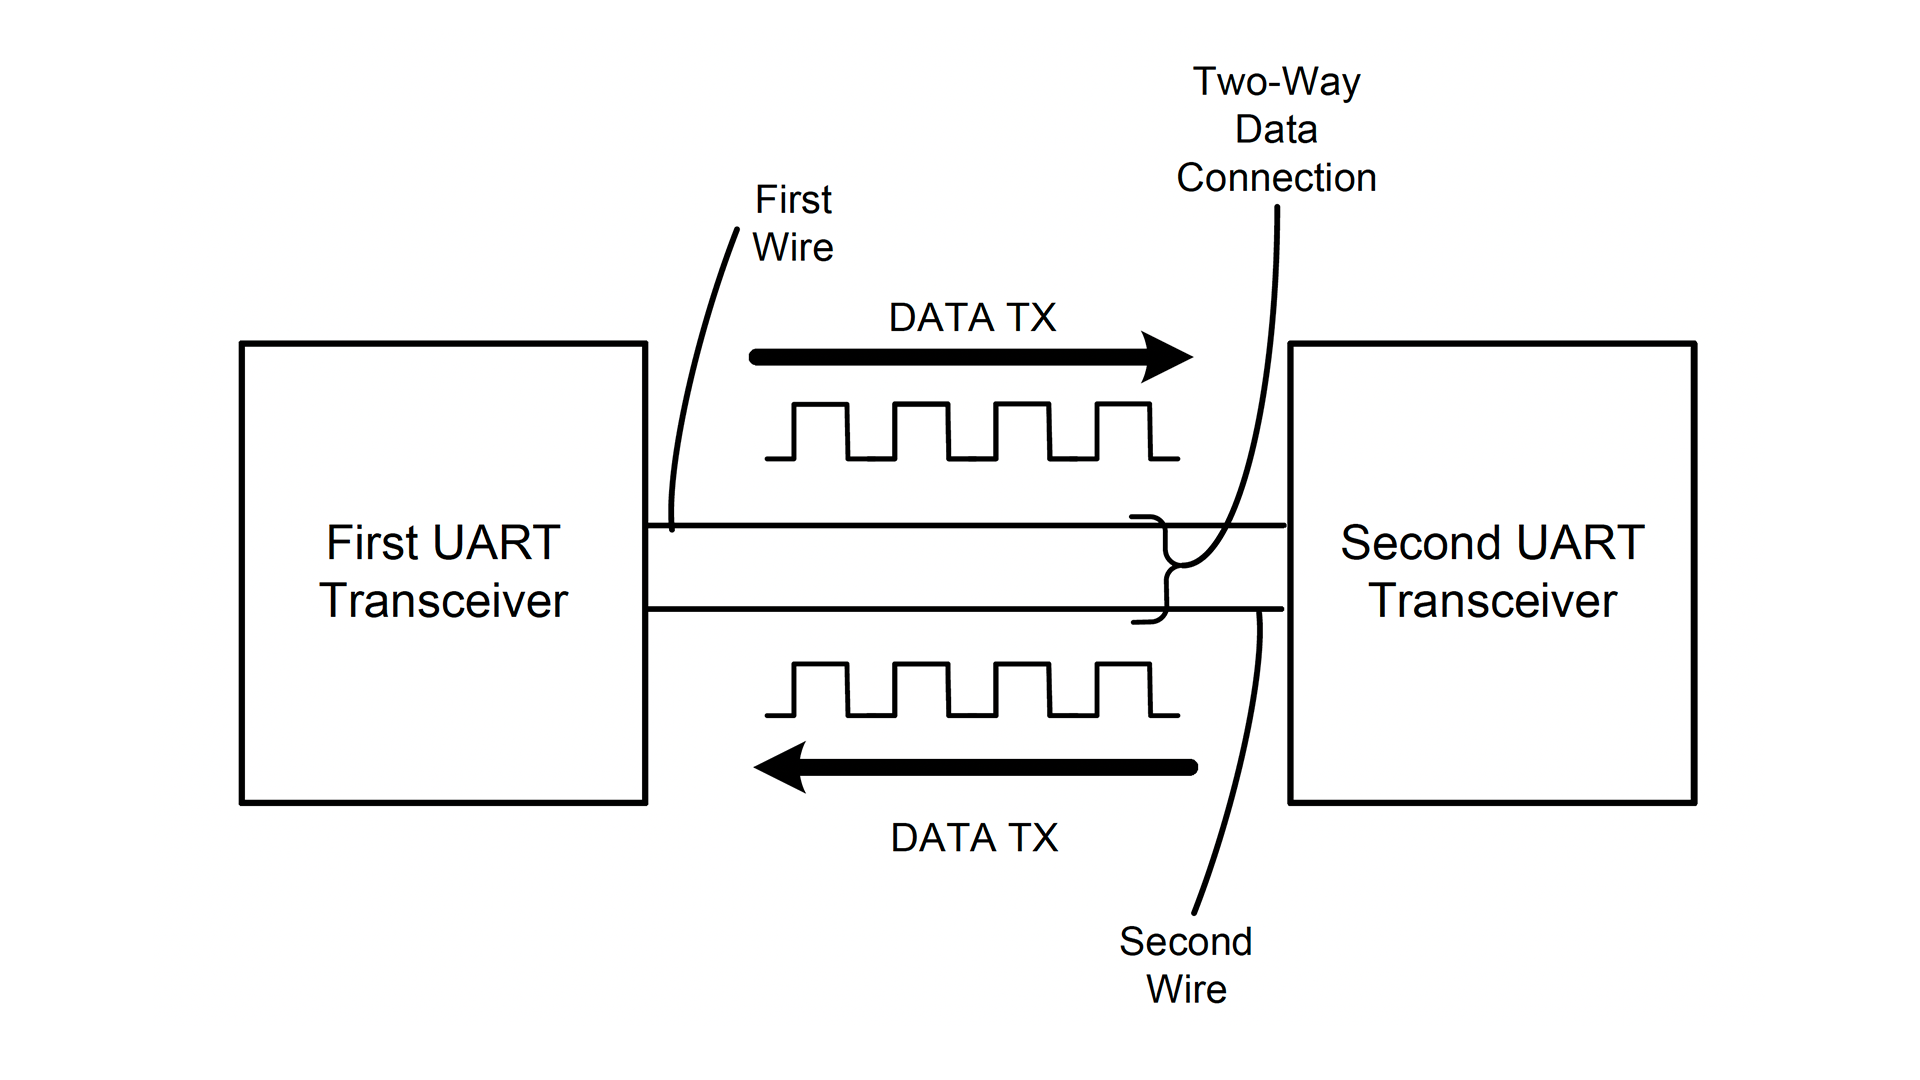
\includegraphics[width=0.6\textwidth]{img/fig41-Wired-UART.png} 
    \caption{Giao thức truyền thông UART}
    \label{fig41}
    \vspace{0.2cm}
\end{figure}

\subsection{Phân tích thời gian truyền thông UART}

Việc phân tích thời gian truyền thông trên bus UART là cần thiết để đảm bảo tốc độ cập nhật lệnh servo đáp ứng yêu cầu thời gian thực của vòng lặp điều khiển. Với baudrate 1 Mbps và giao thức bán song công (half-duplex), mỗi giao dịch bao gồm:

\begin{itemize}
    \item \textbf{Gói lệnh ghi (Write):} Gồm header (2 byte), ID servo (1 byte), chiều dài (1 byte), lệnh (1 byte), dữ liệu vị trí + tốc độ (4 byte), và checksum (1 byte). Tổng: 10 byte.
    \item \textbf{Gói phản hồi (Response):} Gồm header (2 byte), ID (1 byte), chiều dài (1 byte), lỗi (1 byte), dữ liệu (2 byte), và checksum (1 byte). Tổng: 8 byte.
\end{itemize}

Với cấu hình 8N1 (8 bit dữ liệu, không parity, 1 stop bit), mỗi byte cần 10 bit truyền. Thời gian cho một giao dịch hoàn chỉnh (ghi + đọc) với một servo:

\begin{equation}
    t_{servo} = \frac{(10 + 8) \times 10}{10^6} = 180 \; \mu\text{s}
\end{equation}

Mỗi bus driver quản lý 6 servo, thời gian tổng cho một frame lệnh:

\begin{equation}
    t_{bus} = 6 \times t_{servo} = 6 \times 180 = 1080 \; \mu\text{s} \approx 1{,}1 \text{ ms}
\end{equation}

Hai bus hoạt động song song trên hai cổng USB riêng biệt, nên tổng thời gian truyền thông cho 12 servo vẫn xấp xỉ $1{,}1$ ms --- nhỏ hơn nhiều so với chu kỳ điều khiển $\Delta T = 7$ ms. Điều này xác nhận băng thông truyền thông đủ cho vận hành thời gian thực.

\subsection{Ánh xạ ID servo và phân bổ driver}

Bảng~\ref{tab:servo_mapping} trình bày cấu hình ánh xạ ID servo và phân bổ cho hai driver UART.

\begin{table}[H]
\centering
\caption{Ánh xạ ID servo theo driver và chân robot}
\label{tab:servo_mapping}
\renewcommand{\arraystretch}{1.3}
\begin{tabular}{|l|c|c|c|c|}
\hline
\textbf{Chân} & \textbf{Driver} & \textbf{Hip Roll} & \textbf{Hip Pitch} & \textbf{Knee} \\ \hline
Left-Front (LF) & A & ID 7 & ID 8 & ID 9 \\ \hline
Right-Behind (RB) & A & ID 10 & ID 11 & ID 12 \\ \hline
Right-Front (RF) & B & ID 1 & ID 2 & ID 3 \\ \hline
Left-Behind (LB) & B & ID 4 & ID 5 & ID 6 \\ \hline
\end{tabular}
\end{table}

Chiến lược phân bổ ghép hai chân \textit{chéo nhau} trên cùng một driver (LF+RB trên Driver A, RF+LB trên Driver B) có ý nghĩa quan trọng: trong dáng đi Trot, hai chân chéo luôn ở cùng pha (swing hoặc stance). Khi một cặp chéo đang ở pha swing (cần cập nhật vị trí nhanh), cặp còn lại ở pha stance (ít thay đổi), giúp cân bằng tải truyền thông giữa hai bus.

\section{Kiến trúc phần mềm ROS 2}

\subsection{Tổng quan kiến trúc node}

Hệ thống phần mềm được triển khai trên nền tảng ROS~2 Humble \cite{ros2docs}, sử dụng kiến trúc xử lý phân tán gồm hai node tính toán được phân vùng theo chức năng:

\begin{itemize}
    \item \textbf{Gait Generator Node:} Quản lý toàn bộ quá trình tính toán quỹ đạo tuần hoàn, giải bài toán động học nghịch và gửi lệnh điều khiển đến các cơ cấu chấp hành qua bus nối tiếp. Node này được lập trình bằng Python, bao gồm các module: \texttt{gaitGenerator.py} (37KB -- tạo dáng đi), \texttt{kinematics.py} (IK solver), \texttt{quinticPlanning.py} (nội suy đa thức bậc 5) và \texttt{serialPublish.py} (giao tiếp UART với servo).
    
    \item \textbf{Balance Controller Node:} Xử lý bất đồng bộ việc thu thập dữ liệu quán tính tần số cao, xử lý tín hiệu đa giai đoạn và tính toán bù PID. Node này hoạt động độc lập qua module \texttt{nodeBalanceController.py} (22KB).
\end{itemize}

\subsection{Giao tiếp giữa các node}

Giao tiếp liên tiến trình giữa hai node sử dụng cơ chế publish-subscribe qua DDS (Data Distribution Service) của ROS~2. Balance Controller node phát các thông điệp vector hiệu chỉnh nhẹ trên các topic bất đồng bộ chuyên dụng. Kiến trúc tách rời này đảm bảo rằng các nút thắt xử lý tại Gait Generator không thể chiếm quyền hoặc chặn các bù trừ cảm biến quan trọng, cho phép vận hành xác định, chịu lỗi ngay cả dưới tải CPU cao.

Sơ đồ tổng thể kiến trúc ROS~2 bao gồm các node, topic và luồng dữ liệu giữa các thành phần được thể hiện trong Hình~\ref{fig:ros2_arch}. Sơ đồ phân biệt rõ các thành phần theo loại: ROS~2 node (Python), driver (C++), topic truyền thông, cảm biến phần cứng, và giao diện mô phỏng Gazebo.

\begin{figure}[H]
    \centering
    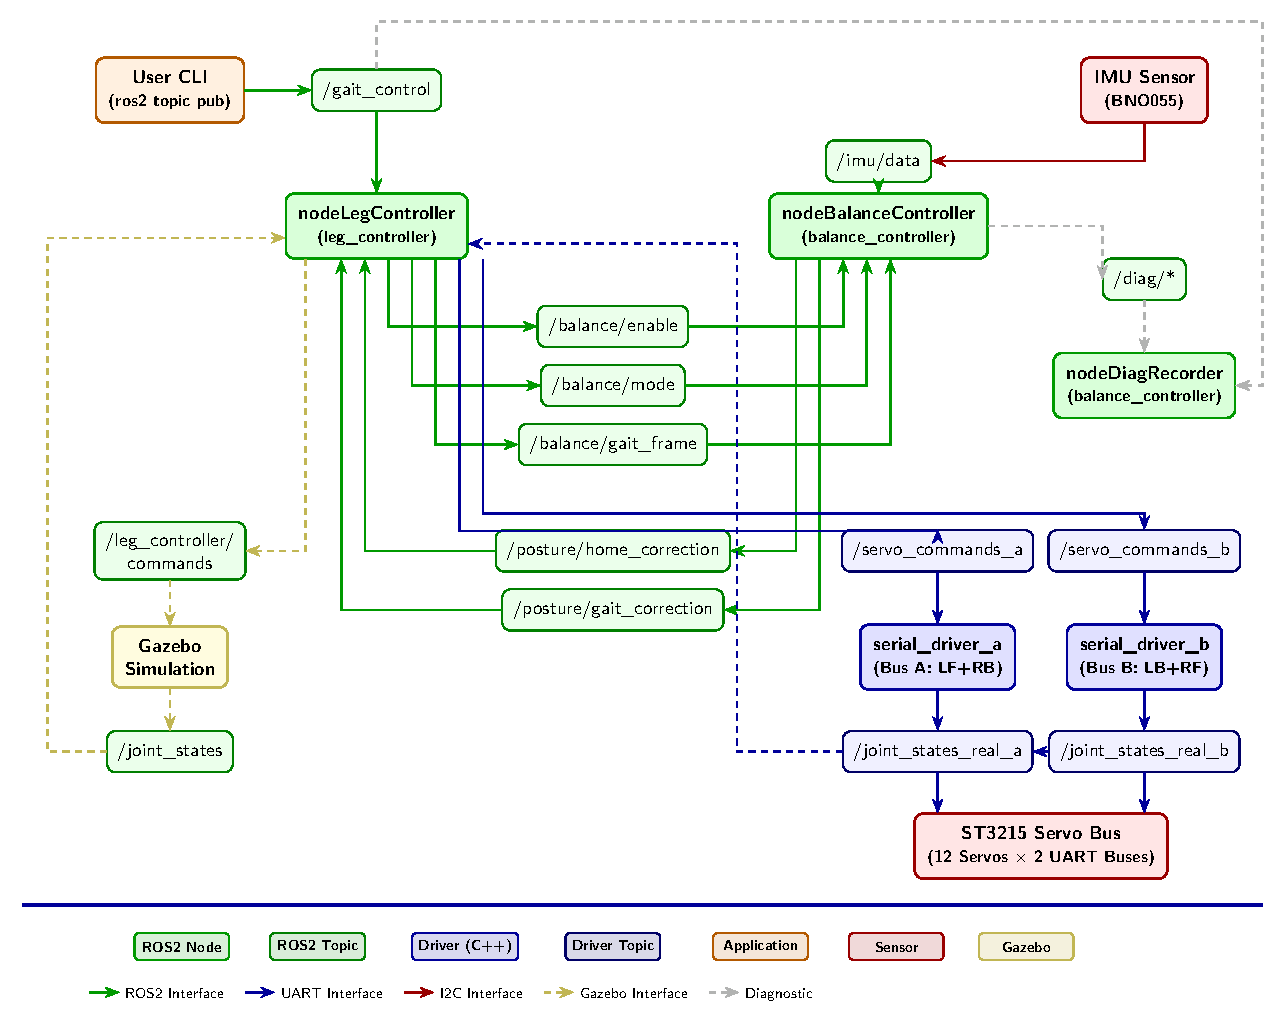
\includegraphics[width=\textwidth]{img/fig_ros2_architecture.pdf}
    \caption{Sơ đồ kiến trúc ROS~2 của hệ thống: các node, topic và luồng dữ liệu}
    \label{fig:ros2_arch}
\end{figure}

\subsection{Các trạng thái vận hành}

Hệ thống quản lý hai trạng thái vận hành rời rạc thông qua cổng logic boolean:

\begin{itemize}
    \item \textbf{HOME:} Cấu hình tĩnh không có vector tịnh tiến tuần hoàn. Bộ điều khiển tính toán các điều chỉnh đồng nhất trong không gian khớp, ánh xạ cứng đến tư thế nghỉ. Sai lệch góc cơ sở được chuyển đổi tỷ lệ thành các bù mô-men đối kháng nhằm hiệu chỉnh tư thế liên tục. Một khoảng trễ khởi động $T_{delay}$ giây có thể cấu hình giúp ngăn hiệu chỉnh sớm trong giai đoạn quá độ khởi tạo hệ thống.
    
    \item \textbf{GAIT:} Trạng thái động kích hoạt khi có lệnh tịnh tiến mặt phẳng. Robot thực hiện quỹ đạo đa thức tuần hoàn sử dụng các mảng dịch pha khả cấu hình để tạo dáng đi trot ($\phi = [0, 0, 0{,}5, 0{,}5]$), walk ($\phi = [0, 0{,}25, 0{,}5, 0{,}75]$) và các dáng đi khác. Các hiệu chỉnh không gian từ phản hồi quán tính chỉ được áp dụng cho chân ở pha chống, trong khi chân ở pha bay duy trì bù bằng không để đảm bảo khoảng trống sải bước.
\end{itemize}

\subsection{Cấu trúc các ROS 2 packages}

Toàn bộ hệ thống phần mềm được tổ chức thành 6 packages ROS~2:

\begin{table}[H]
\centering
\caption{Cấu trúc các ROS 2 packages trong hệ thống}
\label{tab:ros2_packages}
\renewcommand{\arraystretch}{1.3}
\begin{tabular}{|p{0.22\linewidth}|p{0.12\linewidth}|p{0.52\linewidth}|}
\hline
\textbf{Package} & \textbf{Ngôn ngữ} & \textbf{Chức năng} \\ \hline
\texttt{leg\_controller} & Python & Tạo dáng đi, IK solver, quy hoạch quỹ đạo, giao tiếp servo \\ \hline
\texttt{balance\_controller} & Python & Thu thập IMU, xử lý tín hiệu, PID cân bằng, chẩn đoán \\ \hline
\texttt{serial\_driver} & C++ & Driver giao tiếp với bus servo ST3215 (thư viện SCServo) \\ \hline
\texttt{simulation} & Python & Mô hình URDF, cấu hình Gazebo, RViz, launch mô phỏng \\ \hline
\texttt{launch\_main} & CMake & Launch files cho hệ thống thực \\ \hline
\end{tabular}
\end{table}

\subsection{Chi tiết các module phần mềm}

\textbf{Module gaitGenerator.py} là module cốt lõi của hệ thống, quản lý máy trạng thái (state machine) điều khiển toàn bộ vòng đời vận hành của robot. Module này thực hiện các chức năng:

\begin{itemize}
    \item \textbf{Quản lý trạng thái:} Robot chuyển đổi giữa các trạng thái: INIT (khởi tạo) $\rightarrow$ ZERO (homing về tư thế đứng) $\rightarrow$ TROT/WALK/PUSHUP/SWAY (dáng đi) $\rightarrow$ ROBOTOFF (tắt an toàn). Mỗi trạng thái có hàm \texttt{control\_tick()} riêng biệt xử lý một frame điều khiển.
    \item \textbf{Tạo quỹ đạo:} Gọi hàm \texttt{quintic\_planning()} để tạo quỹ đạo hình chữ D cho mỗi chân, sau đó giải IK qua module \texttt{kinematics.py} để chuyển đổi từ tọa độ Đề-các sang góc khớp.
    \item \textbf{Áp dụng hiệu chỉnh IMU:} Nhận tín hiệu bù từ Balance Controller qua hai topic \texttt{/posture/home\_correction} và \texttt{/posture/gait\_correction}, áp dụng vào góc khớp (HOME) hoặc tọa độ bàn chân (GAIT).
    \item \textbf{Xuất lệnh servo:} Gửi góc điều khiển đến module \texttt{serialPublish.py} để chuyển đổi từ góc IK sang góc servo và truyền qua UART.
\end{itemize}

\textbf{Module serialPublish.py} đảm nhận việc chuyển đổi giữa hai chế độ vận hành (mô phỏng và phần cứng thực) thông qua biến cấu hình \texttt{use\_real}:

\begin{itemize}
    \item \textbf{Chế độ mô phỏng:} Xuất bản lệnh mô-men (effort) lên topic \texttt{/effort\_controller/commands} để điều khiển robot trong Gazebo thông qua plugin \texttt{gazebo\_ros2\_control}.
    \item \textbf{Chế độ phần cứng:} Chuyển đổi góc IK sang góc servo bằng các hàm ánh xạ riêng biệt cho từng chân (\texttt{\_ik\_to\_servo\_lf()}, \texttt{\_ik\_to\_servo\_rf()}, v.v.), sau đó xuất bản lên hai topic \texttt{/servo\_commands\_a} và \texttt{/servo\_commands\_b}.
\end{itemize}

\subsection{Bảng giao tiếp topic ROS~2}

Bảng~\ref{tab:ros2_topics} liệt kê các topic chính trong hệ thống, phân loại theo chức năng.

\begin{table}[H]
\centering
\caption{Các topic ROS~2 chính trong hệ thống}
\label{tab:ros2_topics}
\renewcommand{\arraystretch}{1.3}
\begin{tabular}{|p{0.32\linewidth}|p{0.12\linewidth}|p{0.42\linewidth}|}
\hline
\textbf{Topic} & \textbf{Kiểu dữ liệu} & \textbf{Mô tả} \\ \hline
\texttt{/imu/data} & Imu & Dữ liệu quaternion từ BNO055 \\ \hline
\texttt{/balance/enable} & Bool & Bật/tắt bộ PID cân bằng \\ \hline
\texttt{/balance/mode} & String & Chuyển chế độ HOME/GAIT \\ \hline
\texttt{/balance/gait\_frame} & Int32 & Chỉ số frame dáng đi hiện tại \\ \hline
\texttt{/posture/home\_correction} & Vector3 & Tín hiệu bù PID chế độ HOME \\ \hline
\texttt{/posture/gait\_correction} & Vector3 & Tín hiệu bù PID chế độ GAIT \\ \hline
\texttt{/posture/measurement} & Vector3 & Góc roll/pitch đã lọc \\ \hline
\texttt{/servo\_commands\_a} & Float64[] & Lệnh góc cho Driver A (6 servo) \\ \hline
\texttt{/servo\_commands\_b} & Float64[] & Lệnh góc cho Driver B (6 servo) \\ \hline
\end{tabular}
\end{table}

\subsection{Cơ chế chẩn đoán thời gian thực}

Hệ thống tích hợp cơ chế chẩn đoán (diagnostics) cho phép giám sát trực tiếp các biến nội bộ của bộ điều khiển PID trong thời gian thực thông qua công cụ PlotJuggler. Mỗi giai đoạn trong pipeline PID (đo lường $\rightarrow$ sai lệch $\rightarrow$ P/I/D $\rightarrow$ bão hòa $\rightarrow$ lọc) đều có topic chẩn đoán riêng, cho phép:

\begin{itemize}
    \item Quan sát trực tiếp từng thành phần P, I, D và tổng PID
    \item Phát hiện hiện tượng windup hoặc bão hòa đầu ra
    \item So sánh tín hiệu đo (measurement) với điểm đặt (setpoint) để đánh giá chất lượng bám
    \item Ghi lại dữ liệu dưới dạng file CSV để phân tích offline
\end{itemize}

Tổng cộng, hệ thống xuất bản 22 topic chẩn đoán cho chế độ HOME (9 tín hiệu $\times$ 2 trục + 4 tín hiệu áp dụng) và 18 topic cho chế độ GAIT (9 tín hiệu $\times$ 2 trục), cung cấp khả năng quan sát toàn diện đường ống điều khiển.

\section{Quy trình Homing và Calibrate}

\subsection{Calibrate servo}

Trước khi vận hành, mỗi servo cần được calibrate để đảm bảo góc $0^\circ$ cơ học trùng với góc $0^\circ$ trong phần mềm. Quy trình calibrate bao gồm:

\begin{enumerate}
    \item Đặt tất cả chân robot ở tư thế tham chiếu (chân duỗi thẳng, vuông góc với thân).
    \item Đọc vị trí feedback của từng servo qua thư viện SCServo SDK.
    \item Ghi giá trị offset ($\Delta_{calib}$) --- sai lệch giữa vị trí thực tế và vị trí lý thuyết tại góc $0^\circ$.
    \item Lưu offset vào mảng cấu hình trong \texttt{serialPublish.py}, áp dụng tự động trong các lần khởi chạy tiếp theo.
\end{enumerate}

\subsection{Quy trình Homing}

Quy trình homing (đưa robot về tư thế đứng chuẩn) được thực hiện tự động mỗi khi robot khởi động:

\begin{enumerate}
    \item \textbf{Đọc vị trí hiện tại:} Lấy giá trị góc feedback từ tất cả 12 servo ($\theta_{current,i}$).
    \item \textbf{Tính tư thế đích:} Giải IK cho tư thế đứng chuẩn, tạo ra bộ góc đích $\theta_{target,i} = (0^\circ, 0^\circ, 90^\circ)$ cho mỗi chân.
    \item \textbf{Nội suy tuyến tính:} Trong $N_{homing} = 200$ frame, mỗi góc được nội suy tuyến tính:
    \begin{equation}
        \theta_i(k) = \theta_{current,i} + \frac{k}{N_{homing}} (\theta_{target,i} - \theta_{current,i}), \quad k = 0, 1, \ldots, N_{homing}
    \end{equation}
    \item \textbf{Gửi lệnh:} Tại mỗi frame, gửi bộ 12 góc đã nội suy đến servo qua UART.
\end{enumerate}

Phương pháp nội suy tuyến tính đảm bảo chuyển động mượt mà từ bất kỳ vị trí khởi đầu nào, tránh hiện tượng giật hoặc va đập. Tổng thời gian homing: $200 \times 7 = 1400$ ms $\approx 1{,}4$ giây.
\input{chapter/chapter6-mophong}
\input{chapter/chapter7-ketluan}

\begin{thebibliography}{99}

\bibitem{raibert1986}
M.~H. Raibert,
\textit{Legged Robots That Balance}.
MIT Press, Cambridge, MA, 1986.

\bibitem{siciliano2009}
B.~Siciliano, L.~Sciavicco, L.~Villani, and G.~Oriolo,
\textit{Robotics: Modelling, Planning and Control}.
Springer-Verlag, London, 2009.

\bibitem{craig2005}
J.~J. Craig,
\textit{Introduction to Robotics: Mechanics and Control}, 3rd~ed.
Pearson Prentice Hall, 2005.

\bibitem{gonzalez2018}
M.~Gonzalez de Santos, E.~Garcia, and J.~Estremera,
\textit{Quadrupedal Locomotion: An Introduction to the Control of Four-Legged Robots}.
Springer-Verlag, London, 2006.

\bibitem{hyun2014}
D.~J. Hyun, S.~Seok, J.~Lee, and S.~Kim,
``High speed trot-running: Implementation of a hierarchical controller using proprioceptive impedance control on the MIT Cheetah,''
\textit{The International Journal of Robotics Research}, vol.~33, no.~11, pp.~1417--1445, 2014.

\bibitem{bledt2018}
G.~Bledt, M.~J.~Powell, B.~Katz, J.~Di Carlo, P.~M.~Wensing, and S.~Kim,
``MIT Cheetah 3: Design and control of a robust, dynamic quadruped robot,''
in \textit{2018 IEEE/RSJ International Conference on Intelligent Robots and Systems (IROS)}, pp.~2245--2252, 2018.

\bibitem{unitree2021}
Unitree Robotics,
``Go1 -- The future of quadruped robots,''
\url{https://www.unitree.com/go1}, 2021.

\bibitem{gehring2013}
C.~Gehring, S.~Coros, M.~Hutter, M.~Bloesch, M.~A.~Hoepflinger, and R.~Siegwart,
``Control of dynamic gaits for a quadrupedal robot,''
in \textit{2013 IEEE International Conference on Robotics and Automation (ICRA)}, pp.~3287--3292, 2013.

\bibitem{spong2020}
M.~W. Spong, S.~Hutchinson, and M.~Vidyasagar,
\textit{Robot Modeling and Control}, 2nd~ed.
John Wiley \& Sons, 2020.

\bibitem{sandeep2021}
S.~Sandeep, P.~K.~Jain, and S.~C.~Jain,
``Design and development of a quadruped robot,''
\textit{IOP Conf. Ser.: Mater. Sci. Eng.}, vol.~1012, p.~012016, 2021.

\bibitem{ros2docs}
Open Robotics,
``ROS 2 Humble Hawksbill Documentation,''
\url{https://docs.ros.org/en/humble/}, 2022.

\bibitem{gazebo}
Open Robotics,
``Gazebo Classic Simulation,''
\url{http://gazebosim.org/}, 2023.

\bibitem{denavit1955}
J.~Denavit and R.~S. Hartenberg,
``A kinematic notation for lower-pair mechanisms based on matrices,''
\textit{Journal of Applied Mechanics}, vol.~22, no.~2, pp.~215--221, 1955.

\bibitem{marhefka1999}
D.~W. Marhefka and D.~E. Orin,
``Gait planning for energy efficiency in walking machines,''
in \textit{1999 IEEE International Conference on Robotics and Automation (ICRA)}, vol.~1, pp.~474--480, 1999.

\bibitem{hutter2016}
M.~Hutter \textit{et al.},
``ANYmal -- a highly mobile and dynamic quadrupedal robot,''
in \textit{2016 IEEE/RSJ International Conference on Intelligent Robots and Systems (IROS)}, pp.~38--44, 2016.

\bibitem{jetson_nano}
NVIDIA Corporation,
``Jetson Nano Developer Kit -- Technical Specifications,''
\url{https://developer.nvidia.com/embedded/jetson-nano-developer-kit}, 2019.

\bibitem{bno055}
Bosch Sensortec,
``BNO055 Intelligent 9-axis Absolute Orientation Sensor -- Data Sheet,''
Rev.~1.8, 2021.

\bibitem{waveshare_st3215}
Waveshare Electronics,
``ST3215 Serial Bus Servo -- Datasheet,''
\url{https://www.waveshare.com/st3215-servo.htm}, 2023.

\bibitem{madgwick2011}
S.~O.~H. Madgwick, A.~J.~L. Harrison, and R.~Vaidyanathan,
``Estimation of IMU and MARG orientation using a gradient descent algorithm,''
in \textit{Proc. IEEE International Conference on Rehabilitation Robotics}, pp.~1--7, 2011.

\bibitem{astrom2006}
K.~J. \AA{}str\"{o}m and T.~H\"{a}gglund,
\textit{Advanced PID Control}.
ISA --- The Instrumentation, Systems and Automation Society, 2006.

\bibitem{kajita2003}
S.~Kajita \textit{et al.},
``Biped walking pattern generation by using preview control of zero-moment point,''
in \textit{Proc. IEEE International Conference on Robotics and Automation (ICRA)}, vol.~2, pp.~1620--1626, 2003.

\bibitem{li2022}
J.~Li, L.~Ye, Z.~Jin, H.~Liu, and B.~Liang,
``Posture stabilization control for a quadruped robot walking on swaying platforms,''
in \textit{Proc. IEEE 18th International Conference on Automation Science and Engineering (CASE)}, pp.~1--8, 2022.

\end{thebibliography}

\end{document}